%%%%%%%%%%%%%%%%%%%% book.tex %%%%%%%%%%%%%%%%%%%%%%%%%%%%%
%
% sample root file for the chapters of your "monograph"
%
% Use this file as a template for your own input.
%
%%%%%%%%%%%%%%%% Springer-Verlag %%%%%%%%%%%%%%%%%%%%%%%%%%


% RECOMMENDED %%%%%%%%%%%%%%%%%%%%%%%%%%%%%%%%%%%%%%%%%%%%%%%%%%%
%\documentclass[graybox, envcountchap, twocolumn]{styles02/svmono}
\documentclass[norunningheads, graybox, envcountchap]{styles02/svmono}
\usepackage[a4paper, 
left=20mm,
right=20mm,
top=20mm,
bottom=20mm,
%headheight=50mm
footskip=5mm
]{geometry}

%\usepackage{bookmark}
% set indent to be 0
\setlength{\parindent}{0pt}
%==========================================
% chapter title formating
\usepackage{titlesec}
\titleformat{\chapter}[display]
{\normalfont\Huge \scshape}{\titlerule}{-28pt}{\thechapter\ \ \Huge}[\vspace{-2pt}\titlerule]
\titleformat{name=\chapter,numberless}[display]
{\normalfont\Huge \scshape}{\titlerule}{-28pt}{\Huge}[\vspace{-2pt}\titlerule]
\titlespacing*{\chapter}{0pt}{0pt}{20pt}

%==========================================
% head and foot formating
\usepackage{fancyhdr}
\pagestyle{fancy}
%\fancyhf{}
\setlength\headheight{15pt} 
%\fancyfoot[R]{\thepage}
%==========================================

%\textwidth of 117 mm or 27-3/4 pi pi 
%a \textheight of 191 mm or 45-1/6 pi 
%a \headsep of 12 pt (space between the running head and text).

% choose options for [] as required from the list
% in the Reference Guide

%==========================================
% Adding Parts
%
\usepackage{tocloft}

\makeatletter
\@addtoreset{section}{part}
\makeatother
\newlength\mylen
\renewcommand\thepart{\arabic{part}}
\renewcommand\cftpartpresnum{Part~}
\settowidth\mylen{\bfseries\cftpartpresnum\cftpartaftersnum}
\addtolength\cftpartnumwidth{\mylen}

%==========================================
%%%%%%%%%%%%%%%%%%%%%%%%%%%%%%%%%%%%%%%%%%%%%%%%%%%%%%%%%%%%%%%%%
% graybox example
%\begin{svgraybox}...\end{svgraybox
%%%%%%%%%%%%%%%%%%%%%%%%%%%%%%%%%%%%%%%%%%%%%%%%%%%%%%%%%%%%%%%%%

%
\usepackage{type1cm}         

\usepackage{makeidx}         % allows index generation
\usepackage{graphicx}        % standard LaTeX graphics tool
% when including figure files
\usepackage{multicol}        % used for the two-column index
\usepackage[bottom]{footmisc}% places footnotes at page bottom

% see the list of further useful packages
% in the Reference Guide

% please use the style svind.ist with
% your makeindex program

%%%%%%%%%%%%%%%%%%%%%%%%%%%%%%%%%%%%%%%%%%%%%%%%%%%%%%%%%%%%%%%%%%%%%

\usepackage{amssymb,amsmath,bm}
\DeclareMathAlphabet{\mathcal}{OMS}{cmsy}{m}{n}
\usepackage{textcomp}
\newcommand\abs[1]{\left\lvert#1\right\rvert}
\usepackage{longtable}
\usepackage{algorithm2e}
\usepackage{tocbibind}
\usepackage[toc]{multitoc}
\renewcommand{\bibname}{References}

%%----------------------------------------------------------------------------
\usepackage{mathptmx}        % selects Times Roman as basic font
\usepackage{helvet}          % selects Helvetica as sans-serif font
\usepackage{courier}         % selects Courier as typewriter font
%\usepackage{type1cm}        % activate if the above 3 fonts are 
% not available on your system

% when including figure files
\usepackage[justification=centering]{caption}
\usepackage{subfig}
\usepackage{multirow}
\usepackage[
bookmarksnumbered=true,
bookmarksopen=true,
%bookmarks=true
colorlinks=true,
linkcolor=blue,
anchorcolor=blue,
citecolor=blue
]{hyperref}

\graphicspath{{figures/}}

% see the list of further useful packages in the Reference Guide

\makeindex             % used for the subject index
% please use the style svind.ist with
% your makeindex program

\begin{document}
	
%	\author{soulmachine@gmail.com}
%	\title{Machine Learning Cheat Sheet}
%	\subtitle{Classical equations, diagrams and tricks in machine learning}
	\author{Huafeng Sheng}
	\title{Machine Learning Notebook}
	\subtitle{-- Personalized Edition}
	\maketitle
	
	\frontmatter%%%%%%%%%%%%%%%%%%%%%%%%%%%%%%%%%%%%%%%%%%%%%%%%%%%%%%
	
%	\onecolumn
\begin{titlepage}

{\large Link to Orginal Cheat Sheet:}\\
\url{https://github.com/soulmachine/machine-learning-cheat-sheet}

\end{titlepage}

\newpage

\noindent \textcopyright  2013 soulmachine \\
Except where otherwise noted, This document is licensed under a Creative Commons 
Attribution-ShareAlike 3.0 Unported (CC BY-SA3.0) license \\ (\url{http://creativecommons.org/licenses/by/3.0/}).

	%\include{dedic}
	%\include{foreword}
	\include{preface}
	%\include{acknow}
	
	\tableofcontents
	%\include{acronym}
	\include{notation}
	
	
	\mainmatter%%%%%%%%%%%%%%%%%%%%%%%%%%%%%%%%%%%%%%%%%%%%%%%%%%%%%%%
	\part{Supervised Learning and Unsupervised Learning}
	\chapter{Introduction}

\section{Types of machine learning}
\begin{equation}\nonumber
\begin{cases}
\text{Supervised learning} \begin{cases} \text{Classification} \\ \text{Regression} \end{cases}\\
\text{Unsupervised learning} \begin{cases} \text{Discovering clusters} \\ \text{Discovering latent factors} \\ \text{Discovering graph structure} \\ \text{Matrix completion} \end{cases}\\
\end{cases}
\end{equation}


\section{Three elements of a machine learning model}

\textbf{Model = Representation + Evaluation + Optimization}\footnote{Domingos, P. A few useful things to know about machine learning. Commun. ACM. 55(10):78–87 (2012).}


\subsection{Representation}
In supervised learning, a model must be represented as a conditional probability distribution $P(y|\vec{x})$(usually we call it classifier) or a decision function $f(x)$. The set of classifiers(or decision functions) is called the hypothesis space of the model. Choosing a representation for a model is tantamount to choosing the hypothesis space that it can possibly learn. 


\subsection{Evaluation}
In the hypothesis space, an evaluation function (also called objective function or risk function) is needed to distinguish good classifiers(or decision functions) from bad ones.


\subsubsection{Loss function and risk function}
\label{sec:Loss-function-and-risk-function}

\begin{definition}
In order to measure how well a function fits the training data, a \textbf{loss function} $L:Y \times Y \rightarrow R \geq 0$ is defined. For training example $(x_i,y_i)$, the loss of predicting the value $\widehat{y}$ is $L(y_i,\widehat{y})$.
\end{definition}

The following is some common loss functions:
\begin{enumerate}
\item 0-1 loss function \\ $L(Y,f(X))=\mathbb{I}(Y,f(X))=\begin{cases} 1, & Y=f(X) \\ 0, & Y \neq f(X) \end{cases}$
\item Quadratic loss function $L(Y,f(X))=\left(Y-f(X)\right)^2$
\item Absolute loss function $L(Y,f(X))=\abs{Y-f(X)}$
\item Logarithmic loss function \\ $L(Y,P(Y|X))=-\log{P(Y|X)}$
\end{enumerate}

\begin{definition}
The risk of function $f$ is defined as the expected loss of $f$:
\begin{equation}\label{eqn:expected-loss}
R_{\mathrm{exp}}(f)=E\left[L\left(Y,f(X)\right)\right]=\int L\left(y,f(x)\right)P(x,y)\mathrm{d}x\mathrm{d}y
\end{equation}
which is also called expected loss or \textbf{risk function}.
\end{definition}

\begin{definition}
The risk function $R_{\mathrm{exp}}(f)$ can be estimated from the training data as
\begin{equation}
R_{\mathrm{emp}}(f)=\dfrac{1}{N}\sum\limits_{i=1}^{N} L\left(y_i,f(x_i)\right)
\end{equation}
which is also called empirical loss or \textbf{empirical risk}.
\end{definition}

You can define your own loss function, but if you're a novice, you're probably better off using one from the literature. There are conditions that loss functions should meet\footnote{\url{http://t.cn/zTrDxLO}}:
\begin{enumerate}
\item They should approximate the actual loss you're trying to minimize. As was said in the other answer, the standard loss functions for classification is zero-one-loss (misclassification rate) and the ones used for training classifiers are approximations of that loss.
\item The loss function should work with your intended optimization algorithm. That's why zero-one-loss is not used directly: it doesn't work with gradient-based optimization methods since it doesn't have a well-defined gradient (or even a subgradient, like the hinge loss for SVMs has).

The main algorithm that optimizes the zero-one-loss directly is the old perceptron algorithm(chapter \S \ref{chap:Perceptron}).
\end{enumerate}


\subsubsection{ERM and SRM}
\begin{definition}
ERM(Empirical risk minimization)
\begin{equation}
\min\limits _{f \in \mathcal{F}} R_{\mathrm{emp}}(f)=\min\limits _{f \in \mathcal{F}} \dfrac{1}{N}\sum\limits_{i=1}^{N} L\left(y_i,f(x_i)\right)
\end{equation}
\end{definition}

\begin{definition}
Structural risk
\begin{equation}
R_{\mathrm{smp}}(f)=\dfrac{1}{N}\sum\limits_{i=1}^{N} L\left(y_i,f(x_i)\right) +\lambda J(f)
\end{equation}
\end{definition}

\begin{definition}
SRM(Structural risk minimization)
\begin{equation}
\min\limits _{f \in \mathcal{F}} R_{\mathrm{srm}}(f)=\min\limits _{f \in \mathcal{F}} \dfrac{1}{N}\sum\limits_{i=1}^{N} L\left(y_i,f(x_i)\right) +\lambda J(f)
\end{equation}
\end{definition}


\subsection{Optimization}
Finally, we need a \textbf{training algorithm}(also called \textbf{learning algorithm}) to search among the classifiers in the the hypothesis space for the highest-scoring one. The choice of optimization technique is key to the \textbf{efficiency} of the model.


\section{Some basic concepts}


\subsection{Parametric vs non-parametric models}


\subsection{A simple non-parametric classifier: K-nearest neighbours}

\subsubsection{Representation}
\begin{equation}
y=f(\vec{x})=\arg\min_{c}{\sum\limits_{\vec{x}_i \in N_k(\vec{x})} \mathbb{I}(y_i=c)}
\end{equation}
where $N_k(\vec{x})$ is the set of k points that are closest to point $\vec{x}$.

Usually use \textbf{k-d tree} to accelerate the process of finding k nearest points.

\subsubsection{Evaluation}
No training is needed.

\subsubsection{Optimization}
No training is needed.


\subsection{Overfitting}


\subsection{Cross validation}
\label{sec:Cross-validation}
\begin{definition}
\textbf{Cross validation}, sometimes called \emph{rotation estimation}, is a \emph{model validation} technique for assessing how the results of a statistical analysis will generalize to an independent data set\footnote{\small{\url{http://en.wikipedia.org/wiki/Cross-validation_(statistics)}}}.
\end{definition}

Common types of cross-validation:
\begin{enumerate}
\item K-fold cross-validation. In k-fold cross-validation, the original sample is randomly partitioned into k equal size subsamples. Of the k subsamples, a single subsample is retained as the validation data for testing the model, and the remaining k − 1 subsamples are used as training data.
\item 2-fold cross-validation. Also, called simple cross-validation or holdout method. This is the simplest variation of k-fold cross-validation, k=2.
\item Leave-one-out cross-validation(\emph{LOOCV}). k=M, the number of original samples.
\end{enumerate}


\subsection{Model selection}
When we have a variety of models of different complexity (e.g., linear or logistic regression models with different degree polynomials, or KNN classifiers with different values ofK), how should we pick the right one? A natural approach is to compute the \textbf{misclassification rate} on the training set for each method.



	\chapter{Probability}

\section{Frequentists vs. Bayesians}
what is probability? 

One is called the \textbf{frequentist} interpretation. In this view, probabilities represent long run frequencies of events. For example, the above statement means that, if we flip the coin many times, we expect it to land heads about half the time.

The other interpretation is called the \textbf{Bayesian} interpretation of probability. In this view, probability is used to quantify our \textbf{uncertainty} about something; hence it is fundamentally related to information rather than repeated trials (Jaynes 2003). In the Bayesian view, the above statement means we believe the coin is equally likely to land heads or tails on the next toss

One big advantage of the Bayesian interpretation is that it can be used to model our uncertainty about events that do not have long term frequencies. For example, we might want to compute the probability that the polar ice cap will melt by 2020 CE. This event will happen zero or one times, but cannot happen repeatedly. Nevertheless, we ought to be able to quantify our uncertainty about this event. To give another machine learning oriented example, we might have observed a “blip” on our radar screen, and want to compute the probability distribution over the location of the corresponding target (be it a bird, plane, or missile). In all these cases, the idea of repeated trials does not make sense, but the Bayesian interpretation is valid and indeed quite natural. We shall therefore adopt the Bayesian interpretation in this book. Fortunately, the basic rules of probability theory are the same, no matter which interpretation is adopted.


\section{A brief review of probability theory}


\subsection{Basic concepts}
We denote a random event by defining a \textbf{random variable} $X$.

\textbf{Descrete random variable}: $X$ can take on any value from a finite or countably infinite set.

\textbf{Continuous random variable}: the value of $X$ is real-valued.


\subsubsection{CDF}

\begin{equation}
F(x) \triangleq P(X \leq x)=\begin{cases}
\sum_{u \leq x}p(u) & \text{, discrete}\\
\int_{-\infty}^{x} f(u)\mathrm{d}u & \text{, continuous}\\
\end{cases}
\end{equation}


\subsubsection{PMF and PDF}
For descrete random variable, We denote the probability of the event that $X=x$ by $P(X=x)$, or just $p(x)$ for short. Here $p(x)$ is called a \textbf{probability mass function} or \textbf{PMF}.A probability mass function is a function that gives the probability that a discrete random variable is exactly equal to some value\footnote{\url{http://en.wikipedia.org/wiki/Probability_mass_function}}. This satisfies the properties $0 \leq p(x) \leq 1$ and $\sum_{x \in \mathcal{X}} p(x)=1$.

For continuous variable, in the equation $F(x)=\int_{-\infty}^{x} f(u)\mathrm{d}u$, the function $f(x)$ is called a \textbf{probability density function} or \textbf{PDF}. A probability density function is a function that describes the relative likelihood for this random variable to take on a given value\footnote{\url{http://en.wikipedia.org/wiki/Probability_density_function}}.This satisfies the properties $f(x) \geq 0$ and $\int_{-\infty}^{\infty} f(x)\mathrm{d}x=1$.


\subsection{Mutivariate random variables}


\subsubsection{Joint CDF}
We denote joint CDF by $F(x,y) \triangleq P(X \leq x \cap Y \leq y)=P(X \leq x , Y \leq y)$.

\begin{equation}
F(x,y) \triangleq P(X \leq x, Y \leq y)=\begin{cases}
\sum_{u \leq x, v \leq y}p(u,v) \\
\int_{-\infty}^{x}\int_{-\infty}^{y} f(u,v)\mathrm{d}u\mathrm{d}v \\
\end{cases}
\end{equation}

\textbf{product rule}:
\begin{equation}\label{eqn:product-rule}
p(X,Y)=P(X|Y)P(Y)
\end{equation}

\textbf{Chain rule}:
\begin{equation}
p(X_{1:N})=p(X_1)p(X_2|X_1)p(X_3|X_2,X_1)...p(X_N|X_{1:N-1})
\end{equation}


\subsubsection{Marginal distribution}
\textbf{Marginal CDF}:
\begin{equation}\begin{split}
& F_X(x) \triangleq F(x,+\infty)= \\
& \begin{cases}
\sum\limits_{x_i \leq x}P(X=x_i)=\sum\limits_{x_i \leq x}\sum\limits_{j=1}^{+\infty}P(X=x_i,Y=y_j) \\
\int_{-\infty}^{x}f_X(u)du=\int_{-\infty}^{x}\int_{-\infty}^{+\infty} f(u,v)\mathrm{d}u\mathrm{d}v \\
\end{cases}
\end{split}\end{equation}

\begin{equation}\begin{split}
& F_Y(y) \triangleq F(+\infty,y)= \\
& \begin{cases}
\sum\limits_{y_j \leq y}p(Y=y_j)=\sum\limits_{i=1}^{+\infty}\sum_{y_j \leq y}P(X=x_i,Y=y_j) \\
\int_{-\infty}^{y}f_Y(v)dv=\int_{-\infty}^{+\infty}\int_{-\infty}^{y} f(u,v)\mathrm{d}u\mathrm{d}v \\
\end{cases}
\end{split}\end{equation}

\textbf{Marginal PMF and PDF}:
\begin{equation} \begin{cases}
P(X=x_i)=\sum_{j=1}^{+\infty}P(X=x_i,Y=y_j) & \text{, descrete}\\
f_X(x)=\int_{-\infty}^{+\infty} f(x,y)\mathrm{d}y & \text{, continuous}\\
\end{cases}\end{equation}

\begin{equation}\begin{cases}
p(Y=y_j)=\sum_{i=1}^{+\infty}P(X=x_i,Y=y_j) & \text{, descrete}\\
f_Y(y)=\int_{-\infty}^{+\infty} f(x,y)\mathrm{d}x & \text{, continuous}\\
\end{cases}\end{equation}


\subsubsection{Conditional distribution}
\textbf{Conditional PMF}:
\begin{equation}
p(X=x_i|Y=y_j)=\dfrac{p(X=x_i,Y=y_j)}{p(Y=y_j)} \text{ if } p(Y)>0
\end{equation}
The pmf $p(X|Y)$ is called \textbf{conditional probability}.

\textbf{Conditional PDF}:
\begin{equation}
f_{X|Y}(x|y)=\dfrac{f(x,y)}{f_Y(y)}
\end{equation}

\subsection{Bayes rule}
\begin{equation}
\begin{split}
p(Y=y|X=x) & =\dfrac{p(X=x,Y=y)}{p(X=x)} \\
           & =\dfrac{p(X=x|Y=y)p(Y=y)}{\sum_{y'}p(X=x|Y=y')p(Y=y')}
\end{split}
\end{equation}


\subsection{Independence and conditional independence}
We say $X$ and $Y$ are unconditionally independent or marginally independent, denoted $X \perp Y$, if we can represent the joint as the product of the two marginals, i.e.,
\begin{equation}
X \perp Y=P(X,Y)=P(X)P(Y)
\end{equation}

We say $X$ and $Y$ are conditionally independent(CI) given $Z$ if the conditional joint can be written as a product of conditional marginals:
\begin{equation}
X \perp Y|Z=P(X,Y|Z)=P(X|Z)P(Y|Z)
\end{equation}

\subsection{Quantiles}
Since the cdf $F$ is a monotonically increasing function, it has an inverse; let us denote this by $F^{-1}$. If $F$ is the cdf of $X$ , then $F^{-1}(\alpha)$ is the value of $x_{\alpha}$ such that $P(X \leq x_{\alpha})=\alpha$; this is called the $\alpha$ quantile of $F$. The value $F^{-1}(0.5)$ is the \textbf{median} of the distribution, with half of the probability mass on the left, and half on the right. The values $F^{-1}(0.25)$ and $F^{−1}(0.75)$are the lower and upper \textbf{quartiles}.

\subsection{Mean and variance}
The most familiar property of a distribution is its \textbf{mean},or \textbf{expected value}, denoted by $\mu$. For discrete rv’s, it is defined as $\mathbb{E}[X] \triangleq \sum_{x \in \mathcal{X}}xp(x)$, and for continuous rv’s, it is defined as $\mathbb{E}[X] \triangleq \int_{\mathcal{X}}xp(x)\mathrm{d}x$. If this integral is not finite, the mean is not defined (we will see some examples of this later). 

The \textbf{variance} is a measure of the “spread” of a distribution, denoted by $\sigma^2$. This is defined as follows:
\begin{align}
var[X]& =\mathbb{E}[(X-\mu)^2] \\
      & =\int{(x-\mu)^2p(x)\mathrm{d}x} \nonumber \\
      & =\int{x^2p(x)\mathrm{d}x}+{\mu}^2\int{p(x)\mathrm{d}x}-2\mu\int{xp(x)\mathrm{d}x} \nonumber \\
	  & =\mathbb{E}[X^2]-{\mu}^2
\end{align}

from which we derive the useful result
\begin{equation}
\mathbb{E}[X^2]=\sigma^2+{\mu}^2
\end{equation}

The \textbf{standard deviation} is defined as
\begin{equation}
std[X] \triangleq \sqrt{var[X]}
\end{equation}

This is useful since it has the same units as $X$ itself.

\section{Some common discrete distributions}
In this section, we review some commonly used parametric distributions defined on discrete state spaces, both finite and countably infinite.


\subsection{The Bernoulli and binomial distributions}

\begin{definition}
Now suppose we toss a coin only once. Let $X \in \{0,1\}$ be a binary random variable, with probability of “success” or “heads” of $\theta$. We say that $X$ has a \textbf{Bernoulli distribution}. This is written as $X \sim \text{Ber}(\theta)$, where the pmf is defined as 
\begin{equation}
\text{Ber}(x|\theta) \triangleq \theta^{\mathbb{I}(x=1)}(1-\theta)^{\mathbb{I}(x=0)}
\end{equation}
\end{definition}


\begin{definition}
Suppose we toss a coin $n$ times. Let $X \in \{0,1,\cdots,n\}$ be the number of heads. If the probability of heads is $\theta$, then we say $X$ has a \textbf{binomial distribution}, written as $X \sim \text{Bin}(n, \theta)$. The pmf is given by 
\begin{equation}\label{eqn:binomial-pmf}
\text{Bin}(k|n,\theta) \triangleq \dbinom{n}{k}\theta^k(1-\theta)^{n-k}
\end{equation}
\end{definition}


\subsection{The multinoulli and multinomial distributions}

\begin{definition}
The Bernoulli distribution can be used to model the outcome of one coin tosses. To model the outcome of tossing a K-sided dice, let $\vec{x} =(\mathbb{I}(x=1),\cdots,\mathbb{I}(x=K)) \in \{0,1\}^K$ be a random vector(this is called \textbf{dummy encoding} or \textbf{one-hot encoding}), then we say $X$ has a \textbf{multinoulli distribution}(or \textbf{categorical distribution}), written as $X \sim \text{Cat}(\theta)$. The pmf is given by: 
\begin{equation}
p(\vec{x}) \triangleq \prod\limits_{k=1}^K\theta_k^{\mathbb{I}(x_k=1)}
\end{equation}
\end{definition}

\begin{definition}
Suppose we toss a K-sided dice $n$ times. Let $\vec{x} =(x_1,x_2,\cdots,x_K) \in \{0,1,\cdots,n\}^K$ be a random vector, where $x_j$ is the number of times side $j$ of the dice occurs, then we say $X$ has a \textbf{multinomial distribution}, written as $X \sim \text{Mu}(n, \vec{\theta})$. The pmf is given by 
\begin{equation}\label{eqn:multinomial-pmf}
p(\vec{x}) \triangleq \dbinom{n}{x_1 \cdots x_k} \prod\limits_{k=1}^K\theta_k^{x_k}
\end{equation}
where $\dbinom{n}{x_1 \cdots x_k} \triangleq \dfrac{n!}{x_1!x_2! \cdots x_K!}$
\end{definition}

Bernoulli distribution is just a special case of a Binomial distribution with $n=1$, and so is multinoulli distribution as to multinomial distribution. See Table \ref{tab:multinomial-summary} for a summary.

\begin{table}
\caption{Summary of the multinomial and related distributions.}
\label{tab:multinomial-summary}
\centering
\begin{tabular}{llll}
\hline\noalign{\smallskip}
Name & K & n & X \\
\noalign{\smallskip}\svhline\noalign{\smallskip}
Bernoulli & 1 & 1 & $x \in \{0,1\}$ \\
Binomial & 1 & - & $\vec{x} \in \{0,1,\cdots,n\}$ \\
Multinoulli & - & 1 & $\vec{x} \in \{0,1\}^K, \sum_{k=1}^K x_k=1$ \\
Multinomial & - & - & $\vec{x} \in \{0,1,\cdots,n\}^K, \sum_{k=1}^K x_k=n$ \\
\noalign{\smallskip}\hline
\end{tabular}
\end{table} 


\subsection{The Poisson distribution}
\begin{definition}
We say that $X \in \{0,1,2,\cdots\}$ has a \textbf{Poisson distribution} with parameter $\lambda>0$, written as $X \sim \text{Poi}(\lambda)$, if its pmf is
\begin{equation}
p(x|\lambda)=e^{-\lambda}\dfrac{\lambda^x}{x!}
\end{equation}
\end{definition}

The first term is just the normalization constant, required to ensure the distribution sums to 1.

The Poisson distribution is often used as a model for counts of rare events like radioactive decay and traffic accidents. 

\begin{table*}
\caption{Summary of Bernoulli, binomial multinoulli and multinomial distributions.}
\label{tab:Summary-distribution}
\centering
\begin{tabular}{llllll}
\hline\noalign{\smallskip}
Name & Written as & X & $p(x)$(or $p(\vec{x})$) & $\mathbb{E}[X]$ & $\text{var}[X]$ \\
\noalign{\smallskip}\svhline\noalign{\smallskip}
Bernoulli & $X \sim \text{Ber}(\theta)$ & $x \in \{0,1\}$ & $\theta^{\mathbb{I}(x=1)}(1-\theta)^{\mathbb{I}(x=0)}$ & $\theta$ & $\theta(1-\theta)$ \\
Binomial & $X \sim \text{Bin}(n,\theta)$ & $x \in \{0,1,\cdots,n\}$ & $\dbinom{n}{k}\theta^k(1-\theta)^{n-k}$ & $n\theta$ & $n\theta(1-\theta)$ \\
Multinoulli & $X \sim \text{Cat}(\vec{\theta})$ & $\vec{x} \in \{0,1\}^K, \sum_{k=1}^K x_k=1$ & $\prod\limits_{k=1}^K\theta_j^{\mathbb{I}(x_j=1)}$ & - & - \\
Multinomial & $X \sim \text{Mu}(n,\vec{\theta})$ & $\vec{x} \in \{0,1,\cdots,n\}^K, \sum_{k=1}^K x_k=n$ & $\dbinom{n}{x_1 \cdots x_k} \prod\limits_{k=1}^K\theta_j^{x_j}$ & - & - \\
Poisson & $X \sim \text{Poi}(\lambda)$ & $x \in \{0,1,2,\cdots\}$ & $e^{-\lambda}\dfrac{\lambda^x}{x!}$ & $\lambda$ & $\lambda$ \\
\noalign{\smallskip}\hline
\end{tabular}
\end{table*}


\subsection{The empirical distribution}
The \textbf{empirical distribution function}\footnote{\url{http://en.wikipedia.org/wiki/Empirical_distribution_function}}, or \textbf{empirical cdf}, is the cumulative distribution function associated with the empirical measure of the sample. Let $\mathcal{D}=\{x_1,x_2,\cdots,x_N\}$ be a sample set, it is defined as 
\begin{equation}
F_n(x) \triangleq \dfrac{1}{N}\sum\limits_{i=1}^N\mathbb{I}(x_i \leq x)
\end{equation}


\section{Some common continuous distributions}
In this section we present some commonly used univariate (one-dimensional) continuous probability distributions.


\subsection{Gaussian (normal) distribution}

% \begin{table}
% \caption{Summary of Gaussian distribution}
% \centering
% \begin{tabular}{cccccc}
% \hline\noalign{\smallskip}
% Name & Written as & $f(x)$ & $\mathbb{E}[X]$ & mode & $\text{var}[X]$ \\
% \noalign{\smallskip}\svhline\noalign{\smallskip}
% Gaussian distribution & $X \sim \mathcal{N}(\mu,\sigma^2)$ & $\dfrac{1}{\sqrt{2\pi}\sigma}e^{-\frac{1}{2\sigma^2}\left(x-\mu\right)^2}$ & $\mu$ & $\mu$ & $\sigma^2$ \\
% \noalign{\smallskip}\hline
% \end{tabular}
% \end{table} 

\begin{table}
\caption{Summary of Gaussian distribution.}
\centering
\begin{tabular}{cccccc}
\hline\noalign{\smallskip}
Written as & $f(x)$ & $\mathbb{E}[X]$ & mode & $\text{var}[X]$ \\
\noalign{\smallskip}\svhline\noalign{\smallskip}
$X \sim \mathcal{N}(\mu,\sigma^2)$ & $\dfrac{1}{\sqrt{2\pi}\sigma}e^{-\frac{1}{2\sigma^2}\left(x-\mu\right)^2}$ & $\mu$ & $\mu$ & $\sigma^2$ \\
\noalign{\smallskip}\hline
\end{tabular}
\end{table} 

If $X \sim N(0,1)$,we say $X$ follows a \textbf{standard normal} distribution.

The Gaussian distribution is the most widely used distribution in statistics. There are several reasons for this. 
\begin{enumerate}
\item First, it has two parameters which are easy to interpret, and which capture some of the most basic properties of a distribution, namely its mean and variance. 
\item Second,the central limit theorem (Section TODO) tells us that sums of independent random variables have an approximately Gaussian distribution, making it a good choice for modeling residual errors or “noise”. 
\item Third, the Gaussian distribution makes the least number of assumptions (has maximum entropy), subject to the constraint of having a specified mean and variance, as we show in Section TODO; this makes it a good default choice in many cases. 
\item Finally, it has a simple mathematical form, which results in easy to implement, but often highly effective, methods, as we will see. 
\end{enumerate}
See (Jaynes 2003, ch 7) for a more extensive discussion of why Gaussians are so widely used.


\subsection{Student's t-distribution}
\begin{table}
\caption{Summary of Student's t-distribution.}
\centering
\begin{tabular}{cccccc}
\hline\noalign{\smallskip}
Written as & $f(x)$ & $\mathbb{E}[X]$ & mode & $\text{var}[X]$ \\
\noalign{\smallskip}\svhline\noalign{\smallskip}
$X \sim \mathcal{T}(\mu,\sigma^2,\nu)$ & $\dfrac{\Gamma(\frac{\nu+1}{2})}{\sqrt{\nu\pi}\Gamma(\frac{\nu}{2})}\left[1+\dfrac{1}{\nu}\left(\dfrac{x-\mu}{\nu}\right)^2\right]$ & $\mu$ & $\mu$ & $\dfrac{\nu\sigma^2}{\nu-2}$ \\
\noalign{\smallskip}\hline
\end{tabular}
\end{table}
where  $\Gamma(x)$ is the gamma function:
\begin{equation}
\Gamma(x) \triangleq \int_0^\infty t^{x-1}e^{-t}\mathrm{d}t
\end{equation}
$\mu$ is the mean, $\sigma^2>0$ is the scale parameter, and $\nu>0$ is called the \textbf{degrees of freedom}. See Figure \ref{fig:pdfs-for-NTL} for some plots.

\begin{figure}[hbtp]
\centering
\subfloat[]{\includegraphics[scale=.70]{pdfs-for-NTL-a.png}} \\
\subfloat[]{\includegraphics[scale=.70]{pdfs-for-NTL-b.png}}
\caption{(a) The pdf’s for a $\mathcal{N}(0,1)$, $\mathcal{T}(0,1,1)$ and $Lap(0,1/\sqrt{2})$. The mean is 0 and the variance is 1 for both the Gaussian and Laplace. The mean and variance of the Student is undefined when $\nu=1$.(b) Log of these pdf’s. Note that the Student distribution is not log-concave for any parameter value, unlike the Laplace distribution, which is always log-concave (and log-convex...) Nevertheless, both are unimodal.}
\label{fig:pdfs-for-NTL} 
\end{figure}

The variance is only defined if $\nu>2$. The mean is only defined if $\nu>1$.

As an illustration of the robustness of the Student distribution, consider Figure \ref{fig:robustness}. We see that the Gaussian is affected a lot, whereas the Student distribution hardly changes. This is because the Student has heavier tails, at least for small $\nu$(see Figure \ref{fig:pdfs-for-NTL}).

\begin{figure}[hbtp]
\centering
\subfloat[]{\includegraphics[scale=.70]{robustness-a.png}} \\
\subfloat[]{\includegraphics[scale=.70]{robustness-b.png}}
\caption{Illustration of the effect of outliers on fitting Gaussian, Student and Laplace distributions. (a) No outliers (the Gaussian and Student curves are on top of each other). (b) With outliers. We see that the Gaussian is more affected by outliers than the Student and Laplace distributions.}
\label{fig:robustness} 
\end{figure}

If $\nu=1$, this distribution is known as the \textbf{Cauchy} or \textbf{Lorentz} distribution. This is notable for having such heavy tails that the integral that defines the mean does not converge.

To ensure finite variance, we require $\nu>2$. It is common to use $\nu=4$, which gives good performance in a range of problems (Lange et al. 1989). For $\nu \gg 5$, the Student distribution rapidly approaches a Gaussian distribution and loses its robustness properties.


\subsection{The Laplace distribution}
\begin{table}
\caption{Summary of Laplace distribution.}
\centering
\begin{tabular}{cccccc}
\hline\noalign{\smallskip}
Written as & $f(x)$ & $\mathbb{E}[X]$ & mode & $\text{var}[X]$ \\
\noalign{\smallskip}\svhline\noalign{\smallskip}
$X \sim \text{Lap}(\mu,b)$ & $\dfrac{1}{2b}\exp\left(-\dfrac{|x-\mu|}{b}\right)$ & $\mu$ & $\mu$ & $2b^2$ \\
\noalign{\smallskip}\hline
\end{tabular}
\end{table}

Here $\mu$ is a location parameter and $b>0$ is a scale parameter. See Figure \ref{fig:pdfs-for-NTL} for a plot.

Its robustness to outliers is illustrated in Figure \ref{fig:robustness}. It also put mores probability density at 0 than the Gaussian. This property is a useful way to encourage sparsity in a model, as we will see in Section TODO.


\subsection{The gamma distribution}

\begin{table}
\caption{Summary of gamma distribution}
\centering
\begin{tabular}{ccccccc}
\hline\noalign{\smallskip}
Written as & $X$ & $f(x)$ & $\mathbb{E}[X]$ & mode & $\text{var}[X]$ \\
\noalign{\smallskip}\svhline\noalign{\smallskip}
$X \sim \text{Ga}(a,b)$ & $x \in \mathbb{R}^+$ & $\dfrac{b^a}{\Gamma(a)}x^{a-1}e^{-xb}$ & $\dfrac{a}{b}$ & $\dfrac{a-1}{b}$ & $\dfrac{a}{b^2}$ \\
\noalign{\smallskip}\hline
\end{tabular}
\end{table} 

Here $a>0$ is called the shape parameter and $b>0$ is called the rate parameter. See Figure \ref{fig:gamma-distribution} for some plots.

\begin{figure}[hbtp]
\centering
\subfloat[]{\includegraphics[scale=.50]{gamma-distribution-a.png}} \\
\subfloat[]{\includegraphics[scale=.50]{gamma-distribution-b.png}}
\caption{Some Ga$(a, b=1)$ distributions. If $a \leq 1$, the mode is at 0, otherwise it is $>0$.As we increase the rate $b$, we reduce the horizontal scale, thus squeezing everything leftwards and upwards. (b) An empirical pdf of some rainfall data, with a fitted Gamma distribution superimposed.}
\label{fig:gamma-distribution} 
\end{figure}


\subsection{The beta distribution}

\begin{table*}
\caption{Summary of Beta distribution}\label{tab:beta-distribution}
\centering
\begin{tabular}{ccccccc}
\hline\noalign{\smallskip}
Name & Written as & $X$ & $f(x)$ & $\mathbb{E}[X]$ & mode & $\text{var}[X]$ \\
\noalign{\smallskip}\svhline\noalign{\smallskip}
Beta distribution & $X \sim \text{Beta}(a,b)$ & $x \in [0,1]$ & $\dfrac{1}{B(a,b)}x^{a-1}(1-x)^{b-1}$ & $\dfrac{a}{a+b}$ & $\dfrac{a-1}{a+b-2}$ & $\dfrac{ab}{(a+b)^2(a+b+1)}$ \\
\noalign{\smallskip}\hline
\end{tabular}
\end{table*} 

Here $B(a, b)$is the beta function,
\begin{equation}
B(a,b) \triangleq \dfrac{\Gamma(a)\Gamma(b)}{\Gamma(a+b)}
\end{equation}

See Figure \ref{fig:beta-distribution} for plots of some beta distributions. We require  $a, b >0$ to ensure the distribution is integrable (i.e., to ensure $B(a, b)$ exists). If $a=b=1$, we get the uniform distirbution. If $a$ and $b$ are both less than 1, we get a bimodal distribution with “spikes” at 0 and 1; if $a$ and $b$ are both greater than 1, the distribution is unimodal.

\begin{figure}[hbtp]
\centering
    \includegraphics[scale=.60]{beta-distribution.png}
\caption{Some beta distributions.}
\label{fig:beta-distribution} 
\end{figure}


\subsection{Pareto distribution}

\begin{table*}
\caption{Summary of Pareto distribution}
\centering
\begin{tabular}{ccccccc}
\hline\noalign{\smallskip}
Name & Written as & $X$ & $f(x)$ & $\mathbb{E}[X]$ & mode & $\text{var}[X]$ \\
\noalign{\smallskip}\svhline\noalign{\smallskip}
Pareto distribution & $X \sim \text{Pareto}(k,m)$ & $x \geq m$ & $km^kx^{-(k+1)}\mathbb{I}(x \geq m)$ & $\dfrac{km}{k-1} \text{ if } k > 1$ & $m$ & $\dfrac{m^2k}{(k-1)^2(k-2)} \text{ if } k>2$ \\
\noalign{\smallskip}\hline
\end{tabular}
\end{table*} 

The \textbf{Pareto distribution} is used to model the distribution of quantities that exhibit \textbf{long tails}, also called \textbf{heavy tails}.

As $k \rightarrow \infty$, the distribution approaches $\delta(x-m)$. See Figure \ref{fig:Pareto-distribution}(a) for some plots. If we plot the distribution on a log-log scale, it forms a straight line, of the form $\log p(x)=a\log x+c$ for some constants $a$ and $c$. See Figure \ref{fig:Pareto-distribution}(b) for an illustration (this is known as a \textbf{power law}).

\begin{figure}[hbtp]
\centering
\subfloat[]{\includegraphics[scale=.50]{pareto-distribution-a.png}} \\
\subfloat[]{\includegraphics[scale=.50]{pareto-distribution-b.png}}
\caption{(a) The Pareto distribution Pareto$(x|m, k)$ for $m=1$. (b) The pdf on a log-log scale.}
\label{fig:Pareto-distribution} 
\end{figure}


\section{Joint probability distributions}
Given a \textbf{multivariate random variable} or \textbf{random vector} \footnote{\url{http://en.wikipedia.org/wiki/Multivariate_random_variable}} $X \in \mathbb{R}^D$, the \textbf{joint probability distribution}\footnote{\url{http://en.wikipedia.org/wiki/Joint_probability_distribution}} is a probability distribution that gives the probability that each of $X_1, X_2, \cdots,X_D$ falls in any particular range or discrete set of values specified for that variable. In the case of only two random variables, this is called a \textbf{bivariate distribution}, but the concept generalizes to any number of random variables, giving a \textbf{multivariate distribution}.

The joint probability distribution can be expressed either in terms of a \textbf{joint cumulative distribution function} or in terms of a \textbf{joint probability density function} (in the case of continuous variables) or \textbf{joint probability mass function} (in the case of discrete variables). 


\subsection{Covariance and correlation}
\begin{definition}
The \textbf{covariance} between two rv’s $X$ and $Y$ measures the degree to which $X$ and $Y$ are (linearly) related. Covariance is defined as
\begin{equation}
\begin{split}
\mathrm{cov}[X,Y] & \triangleq \mathbb{E}\left[(X-\mathbb{E}[X])(Y-\mathbb{E}[Y])\right] \\
         & =\mathbb{E}[XY]-\mathbb{E}[X]\mathbb{E}[Y]
\end{split}
\end{equation}
\end{definition}

\begin{definition}
If $X$ is a $D$-dimensional random vector, its \textbf{covariance matrix} is defined to be the following symmetric, positive definite matrix:
\begin{align}
\mathrm{cov}[X] & \triangleq \mathbb{E}\left[(X-\mathbb{E}[X])(X-\mathbb{E}[X])^T\right] \\
       &  = \left( \begin{array}{cccc}
           \text{var}[X_1] & \text{Cov}[X_1,X_2] & \cdots & \text{Cov}[X_1,X_D] \\
           \text{Cov}[X_2,X_1] & \text{var}[X_2] & \cdots & \text{Cov}[X_2,X_D] \\
		   \vdots & \vdots & \ddots & \vdots \\
           \text{Cov}[X_D,X_1] & \text{Cov}[X_D,X_2] & \cdots & \text{var}[X_D] \end{array} \right)
\end{align}
\end{definition}

\begin{definition}
The (Pearson) \textbf{correlation coefficient} between $X$ and $Y$ is defined as
\begin{equation}
\text{corr}[X,Y] \triangleq \dfrac{\text{Cov}[X,Y]}{\sqrt{\text{var}[X],\text{var}[Y]}}
\end{equation}
\end{definition}

A \textbf{correlation matrix} has the form
\begin{equation}
\mathbf{R} \triangleq \left( \begin{array}{cccc}
           \text{corr}[X_1,X_1] & \text{corr}[X_1,X_2] & \cdots & \text{corr}[X_1,X_D] \\
           \text{corr}[X_2,X_1] & \text{corr}[X_2,X_2] & \cdots & \text{corr}[X_2,X_D] \\
		   \vdots & \vdots & \ddots & \vdots \\
           \text{corr}[X_D,X_1] & \text{corr}[X_D,X_2] & \cdots & \text{corr}[X_D,X_D] \end{array} \right)
\end{equation}

The correlation coefficient can viewed as a degree of linearity between $X$ and $Y$, see Figure \ref{fig:Correlation-examples}.
\begin{figure*}[hbtp]
\centering
    \includegraphics[scale=.80]{Correlation-examples.png}
\caption{Several sets of $(x, y)$ points, with the Pearson correlation coefficient of $x$ and $y$ for each set. Note that the correlation reflects the noisiness and direction of a linear relationship (top row), but not the slope of that relationship (middle), nor many aspects of nonlinear relationships (bottom). N.B.: the figure in the center has a slope of 0 but in that case the correlation coefficient is undefined because the variance of $Y$ is zero.Source:\url{http://en.wikipedia.org/wiki/Correlation}}
\label{fig:Correlation-examples} 
\end{figure*}

\textbf{Uncorrelated does not imply independent}. For example, let $X \sim U(-1,1)$ and $Y =X^2$. Clearly $Y$ is dependent on $X$(in fact, $Y$ is uniquely determined by $X$), yet one can show that corr$[X, Y]=0$. Some striking examples of this fact are shown in Figure \ref{fig:Correlation-examples}. This shows several data sets where there is clear dependence between $X$ and $Y$, and yet the correlation coefficient is 0. A more general measure of dependence between random variables is mutual information, see Section TODO.


\subsection{Multivariate Gaussian distribution}
\label{sec:MVN}
The \textbf{multivariate Gaussian} or \textbf{multivariate normal}(MVN) is the most widely used joint probability density function for continuous variables. We discuss MVNs in detail in Chapter 4; here we just give some definitions and plots.

The pdf of the MVN in $D$ dimensions is defined by the following:
\begin{equation}
\mathcal{N}(\vec{x}|\vec{\mu},\Sigma) \triangleq \dfrac{1}{(2\pi)^{D/2}|\Sigma|^{1/2}}\exp\left[-\dfrac{1}{2}(\vec{x}-\vec{\mu})^T\Sigma^{-1}(\vec{x}-\vec{\mu})\right]
\end{equation}
where $\vec{\mu}=\mathbb{E}[X] \in \mathbb{R}^D$ is the mean vector, and $\Sigma=\text{Cov}[X]$ is the $D \times D$ covariance matrix. The normalization constant $(2\pi)^{D/2}|\Sigma|^{1/2}$ just ensures that the pdf integrates to 1.

Figure \ref{fig:2d-Gaussions} plots some MVN densities in 2d for three different kinds of covariance matrices. A full covariance matrix has A $D(D+1)/2$ parameters (we divide by 2 since $\Sigma$ is symmetric). A diagonal covariance matrix has $D$ parameters, and has 0s in the off-diagonal terms. A spherical or isotropic covariance,$\Sigma=\sigma^2\vec{I}_D$, has one free parameter.

\begin{figure}[hbtp]
\centering
\subfloat[]{\includegraphics[scale=.60]{2d-Gaussions-a.png}} \\
\subfloat[]{\includegraphics[scale=.60]{2d-Gaussions-b.png}} \\
\subfloat[]{\includegraphics[scale=.60]{2d-Gaussions-c.png}} \\
\subfloat[]{\includegraphics[scale=.60]{2d-Gaussions-d.png}}
\caption{We show the level sets for 2d Gaussians. (a) A full covariance matrix has elliptical contours.(b) A diagonal covariance matrix is an axis aligned ellipse. (c) A spherical covariance matrix has a circular shape. (d) Surface plot for the spherical Gaussian in (c).}
\label{fig:2d-Gaussions} 
\end{figure}


\subsection{Multivariate Student's t-distribution}
A more robust alternative to the MVN is the multivariate Student's t-distribution, whose pdf is given by
\begin{align}
& \mathcal{T}(x|\vec{\mu},\Sigma,\nu) \nonumber \\
& \triangleq \dfrac{\Gamma(\frac{\nu+D}{2})}{\Gamma(\frac{\nu}{2})}\dfrac{|\Sigma|^{-\frac{1}{2}}}{\left(\nu\pi\right)^{\frac{D}{2}}}\left[1+\dfrac{1}{\nu}\left(\vec{x}-\vec{\mu}\right)^T\Sigma^{-1}\left(\vec{x}-\vec{\mu}\right)\right]^{-\frac{\nu+D}{2}} \\
&= \dfrac{\Gamma(\frac{\nu+D}{2})}{\Gamma(\frac{\nu}{2})}\dfrac{|\Sigma|^{-\frac{1}{2}}}{\left(\nu\pi\right)^{\frac{D}{2}}}\left[1+\left(\vec{x}-\vec{\mu}\right)^T\vec{V}^{-1}\left(\vec{x}-\vec{\mu}\right)\right]^{-\frac{\nu+D}{2}}
\end{align}
where $\Sigma$ is called the scale matrix (since it is not exactly the covariance matrix) and $\vec{V}=\nu\Sigma$. This has fatter tails than a Gaussian. The smaller $\nu$ is, the fatter the tails. As $\nu \rightarrow \infty$, the distribution tends towards a Gaussian. The distribution has the following properties
\begin{equation}
\text{mean}=\vec{\mu} \text{ , mode}=\vec{\mu} \text{ , Cov}= \dfrac{\nu}{\nu-2}\Sigma
\end{equation}


\subsection{Dirichlet distribution}
A multivariate generalization of the beta distribution is the \textbf{Dirichlet distribution}, which has
support over the probability simplex, defined by
\begin{equation}
S_K=\left\{\vec{x}:0 \leq x_k \leq 1,\sum\limits_{k=1}^K x_k=1\right\}
\end{equation}

The pdf is defined as follows:
\begin{equation}
\text{Dir}(\vec{x}|\vec{\alpha}) \triangleq \dfrac{1}{B(\vec{\alpha})}\prod\limits_{k=1}^K x_k^{\alpha_k-1}\mathbb{I}(\vec{x} \in S_K)
\end{equation}
where $B(\alpha_1,\alpha_2,\cdots,\alpha_K)$ is the natural generalization of the beta function to $K$ variables:
\begin{equation}
B(\alpha) \triangleq \dfrac{\prod_{k=1}^K \Gamma(\alpha_k)}{\Gamma(\alpha_0)} \text{ where } \alpha_0 \triangleq \sum_{k=1}^K \alpha_k
\end{equation}

Figure \ref{fig:3d-Dirichlet} shows some plots of the Dirichlet when $K=3$, and Figure \ref{fig:5d-Dirichlet} for some sampled probability vectors. We see that $\alpha_0$ controls the strength of the distribution (how peaked it is), and theαkcontrol where the peak occurs. For example, Dir$(1,1,1)$ is a uniform distribution, Dir$(2,2,2)$ is a broad distribution centered at $(1/3,1/3,1/3)$, and Dir$(20,20,20)$ is a narrow distribution centered at $(1/3,1/3,1/3)$.If $\alpha_k < 1$ for all $k$, we get “spikes” at the corner of the simplex.

\begin{figure}[hbtp]
\centering
\subfloat[]{\includegraphics[scale=.50]{3d-Dirichlet-a.png}} \\
\subfloat[]{\includegraphics[scale=.60]{3d-Dirichlet-b.png}} \\
\subfloat[]{\includegraphics[scale=.60]{3d-Dirichlet-c.png}} \\
\subfloat[]{\includegraphics[scale=.60]{3d-Dirichlet-d.png}}
\caption{(a) The Dirichlet distribution when $K=3$ defines a distribution over the simplex, which can be represented by the triangular surface. Points on this surface satisfy $0 \leq \theta_k \leq 1$ and $\sum_{k=1}^K \theta_k=1$. (b) Plot of the Dirichlet density when $\vec{\alpha}=(2,2,2)$. (c) $\vec{\alpha}=(20,2,2)$.}
\label{fig:3d-Dirichlet} 
\end{figure}

\begin{figure}[hbtp]
\centering
\subfloat[$\vec{\alpha}=(0.1,\cdots,0.1)$. This results in very sparse distributions, with many 0s.]{\includegraphics[scale=.50]{5d-Dirichlet-a.png}} \\
\subfloat[$\vec{\alpha}=(1,\cdots,1)$. This results in more uniform (and dense) distributions.]{\includegraphics[scale=.50]{5d-Dirichlet-b.png}}
\caption{Samples from a 5-dimensional symmetric Dirichlet distribution for different parameter values.} 
\label{fig:5d-Dirichlet} 
\end{figure}

For future reference, the distribution has these properties
\begin{equation}\label{eqn:Dirichlet-properties}
\mathbb{E}(x_k)=\dfrac{\alpha_k}{\alpha_0} \text{, mode}[x_k]=\dfrac{\alpha_k-1}{\alpha_0-K} \text{, var}[x_k]=\dfrac{\alpha_k(\alpha_0-\alpha_k)}{\alpha_0^2(\alpha_0+1)}
\end{equation}


\section{Transformations of random variables}
If $\vec{x} \sim P()$ is some random variable, and $\vec{y}=f(\vec{x})$, what is the distribution of $Y$? This is the question we address in this section.


\subsection{Linear transformations}
Suppose $g()$ is a linear function: 
\begin{equation}
g(\vec{x})=A\vec{x}+b
\end{equation}

First, for the mean, we have
\begin{equation}
\mathbb{E}[\vec{y}]=\mathbb{E}[A\vec{x}+b]=A\mathbb{E}[\vec{x}]+b
\end{equation}
this is called the \textbf{linearity of expectation}.

For the covariance, we have
\begin{equation}
\text{Cov}[\vec{y}]=\text{Cov}[A\vec{x}+b]=A\Sigma A^T
\end{equation}


\subsection{General transformations}
\label{sec:General-transformations}
If $X$ is a discrete rv, we can derive the pmf for $y$ by simply summing up the probability mass for all the $x$’s such that $f(x)=y$:
\begin{equation}\label{eqn:transformation-discrete}
p_Y(y)=\sum\limits_{x:g(x)=y}p_X(x)
\end{equation}

If $X$ is continuous, we cannot use Equation \ref{eqn:transformation-discrete} since $p_X(x)$ is a density, not a pmf, and we cannot sum up densities. Instead, we work with cdf’s, and write
\begin{equation}
F_Y(y)=P(Y \leq y)=P(g(X) \leq y)=\int\limits_{g(X) \leq y} f_X(x)\mathrm{d}x
\end{equation}

We can derive the pdf of $Y$ by differentiating the cdf:
\begin{equation}\label{eqn:General-transformations}
f_Y(y)=f_X(x)|\dfrac{dx}{dy}|
\end{equation}

This is called \textbf{change of variables} formula. We leave the proof of this as an exercise. 

For example, suppose $X \sim U(−1,1)$, and $Y=X^2$. Then $p_Y(y)=\dfrac{1}{2}y^{-\frac{1}{2}}$.


\subsubsection{Multivariate change of variables *}
Let $f$ be a function $f:\mathbb{R}^n \rightarrow \mathbb{R}^n$, and let $\vec{y}=f(\vec{x})$. Then its Jacobian matrix $\vec{J}$ is given by
\begin{equation}
\vec{J}_{\vec{x} \rightarrow \vec{y}} \triangleq \frac{\partial \vec{y}}{\partial \vec{x}} \triangleq \left(\begin{array}{ccc}
\frac{\partial y_1}{\partial x_1} & \cdots & \frac{\partial y_1}{\partial x_n} \\
\vdots & \vdots & \vdots \\
\frac{\partial y_n}{\partial x_1} & \cdots & \frac{\partial y_n}{\partial x_n}
\end{array}\right)
\end{equation}
$|\mathrm{det}(\vec{J})|$ measures how much a unit cube changes in volume when we apply $f$.

If $f$ is an invertible mapping, we can define the pdf of the transformed variables using the Jacobian of the inverse mapping $\vec{y} \rightarrow \vec{x}$:
\begin{equation}\label{eqn:Multivariate-transformation}
p_y(\vec{y})=p_x(\vec{x})|\mathrm{det}(\frac{\partial \vec{x}}{\partial \vec{y}})|=p_x(\vec{x})|\mathrm{det}(\vec{J}_{\vec{y} \rightarrow \vec{x}})|
\end{equation}


\subsection{Central limit theorem}
Given $N$ random variables $X_1,X_2,\cdots,X_N$, each variable is \textbf{independent and identically distributed}\footnote{\url{http://en.wikipedia.org/wiki/Independent_identically_distributed}}(\textbf{iid} for short), and each has the same mean $\mu$ and variance $\sigma^2$, then
\begin{equation}
\dfrac{\sum\limits_{i=1}^n X_i-N\mu}{\sqrt{N}\sigma} \sim \mathcal{N}(0,1)
\end{equation}
this can also be written as
\begin{equation}
\dfrac{\bar{X}-\mu}{\sigma/\sqrt{N}} \sim \mathcal{N}(0,1) \quad \text{, where } \bar{X} \triangleq \dfrac{1}{N}\sum\limits_{i=1}^n X_i
\end{equation}


\section{Monte Carlo approximation}
\label{sec:Monte-Carlo-approximation}
In general, computing the distribution of a function of an rv using the change of variables formula can be difficult. One simple but powerful alternative is as follows. First we generate $S$ samples from the distribution, call them $x_1,\cdots,x_S$. (There are many ways to generate such samples; one popular method, for high dimensional distributions, is called Markov chain Monte Carlo or MCMC; this will be explained in Chapter TODO.) Given the samples, we can approximate the distribution of $f(X)$ by using the empirical distribution of $\left\{f(x_s)\right\}_{s=1}^S$. This is called a \textbf{Monte Carlo approximation}\footnote{\url{http://en.wikipedia.org/wiki/Monte_Carlo_method}}, named after a city in Europe known for its plush gambling casinos.

We can use Monte Carlo to approximate the expected value of any function of a random variable. We simply draw samples, and then compute the arithmetic mean of the function applied to the samples. This can be written as follows:
\begin{equation}
\mathbb{E}[g(X)]=\int g(x)p(x)\mathrm{d}x \approx \dfrac{1}{S}\sum\limits_{s=1}^S f(x_s)
\end{equation}
where $x_s \sim p(X)$.

This is called \textbf{Monte Carlo integration}\footnote{\url{http://en.wikipedia.org/wiki/Monte_Carlo_integration}}, and has the advantage over numerical integration (which is based on evaluating the function at a fixed grid of points) that the function is only evaluated in places where there is non-negligible probability.


\section{Information theory}

\subsection{Entropy}
\label{sec:Entropy}
The entropy of a random variable $X$ with distribution $p$, denoted by $\mathbb{H}(X)$ or sometimes $\mathbb{H}(p)$, is a measure of its uncertainty. In particular, for a discrete variable with $K$ states, it is defined by
\begin{equation}
\mathbb{H}(X) \triangleq -\sum\limits_{k=1}^{K}{p(X=k)\log_2p(X=k)}
\end{equation}

Usually we use log base 2, in which case the units are called \textbf{bits}(short for binary digits). If we use log base $e$ , the units are called \textbf{nats}. 

The discrete distribution with maximum entropy is the uniform distribution (see Section XXX for a proof). Hence for a K-ary random variable, the entropy is maximized if $p(x = k)=1/K$; in this case, $\mathbb{H}(X)=\log_2K$. 

Conversely, the distribution with minimum entropy (which is zero) is any \textbf{delta-function} that puts all its mass on one state. Such a distribution has no uncertainty.


\subsection{KL divergence}
One way to measure the `\textbf{difference}' of two probability distributions, $p$ and $q$ , is known as the \textbf{Kullback-Leibler divergence}(\textbf{KL divergence})or \textbf{relative entropy}: 
%\newpage KL divergence is defined as follows:\\
%\vspace{-15pt}
\begin{flalign}
%	&\mathbb{KL}(Q||P) &\equiv\langle \log q(x)-\log p(x) \rangle _{q(x)} \geq 0 &\\
	\mathbb{KL}(Q||P) &\equiv\langle \log q(x)-\log p(x)\rangle _{q(x)} \geq 0 \\
	&= \mathbb{E}_{q(x)} \big[\log q(x)-\log p(x) \big]\\
	&= \sum \limits_{x}{q(x)\log\dfrac{q(x)}{p(x)}}
\end{flalign}

where the sum gets replaced by an integral for pdfs\footnote{The KL divergence is not a distance, since it is asymmetric. One symmetric version of the KL divergence is the \textbf{Jensen-Shannon divergence}, defined as $JS(p_1,p_2)=0.5\mathbb{KL}(p_1||q)+0.5\mathbb{KL}(p_2||q)$,where $q=0.5p_1+0.5p_2$}. The KL divergence is only defined if P and Q both sum to 1 and if $p(x)=0$ implies $q(x)=0$ for all $x$(absolute continuity). (If the quantity  $0\ln0$ appears in the formula, it is interpreted as zero because $\lim\limits_{x \to 0}x\ln x$.) We can rewrite this as
\begin{equation}\begin{split}
\mathbb{KL}(p||q) & \triangleq \sum\limits_{x}{q(x)\log q(x)}-\sum\limits_{x}{q(x)\log p(x)} \\
    & =\mathbb{H}(q, p)-\mathbb{H}(q)
\end{split}\end{equation}

where $\mathbb{H}(q, p)$ is called the {\color{cyan}\textbf{cross entropy}},
\begin{equation}\label{eqn:cross-entropy}
\mathbb{H}(q, p)=-\sum\limits_{x}{q(x)\log p(x)}
\end{equation}

One can show (Cover and Thomas 2006) that the cross entropy is the average number of bits needed to encode data coming from a source with distribution $q$ when we use model $p$ to define our codebook. Hence the “regular” entropy $\mathbb{H}(q)=\mathbb{H}(q,q)$, defined in section \S \ref{sec:Entropy},is the expected number of bits if we use the true model, so the KL divergence is the diference between these. In other words, the KL divergence is the average number of \emph{extra} bits needed to encode the data, due to the fact that we used distribution $p$ to encode the data instead of the true distribution $q$.

The “extra number of bits” interpretation should make it clear that $\mathbb{KL}(q||p) \geq 0$, and that the KL is only equal to zero if $q = p$. We now give a proof of this important result.

\begin{theorem}
\textbf{Information inequality:} 
\begin{center}
$\mathbb{KL}(p||q) \geq 0 \text{ with equality iff } p=q$.
\end{center}
\end{theorem}

One important consequence of this result is that \emph{the discrete distribution with the maximum
entropy is the uniform distribution}.


\subsection{Mutual information}
\label{sec:Mutual-information}
\begin{definition}
\textbf{Mutual information} or \textbf{MI}, is defined as follows:
\begin{equation}\begin{split}
\mathbb{I}(X;Y) & \triangleq \mathbb{KL}(P(X,Y)||P(X)P(Y)) \\
    & =\sum\limits_x\sum\limits_yp(x,y)\log\dfrac{p(x,y)}{p(x)p(y)}
\end{split}\end{equation}
We have $\mathbb{I}(X;Y) \geq 0$ with equality if $P(X,Y)=P(X)P(Y)$. That is, the MI is zero if the variables are independent.
\end{definition}

To gain insight into the meaning of MI, it helps to re-express it in terms of joint and conditional entropies. One can show that the above expression is equivalent to the following:
\begin{eqnarray}
\mathbb{I}(X;Y)&=&\mathbb{H}(X)-\mathbb{H}(X|Y)\\
               &=&\mathbb{H}(Y)-\mathbb{H}(Y|X)\\
               &=&\mathbb{H}(X)+\mathbb{H}(Y)-\mathbb{H}(X,Y)\\
               &=&\mathbb{H}(X,Y)-\mathbb{H}(X|Y)-\mathbb{H}(Y|X)
\end{eqnarray}
where $\mathbb{H}(X)$ and $\mathbb{H}(Y)$ are the \textbf{marginal entropies}, $\mathbb{H}(X|Y)$ and $\mathbb{H}(Y|X)$ are the \textbf{conditional entropies}, and $\mathbb{H}(X,Y)$ is the \textbf{joint entropy} of $X$ and $Y$, see Fig. \ref{fig:mi}\footnote{\url{http://en.wikipedia.org/wiki/Mutual_information}}.

\begin{figure}[hbtp]
\centering
    \includegraphics[scale=.25]{mutual-information.png}
\caption{Individual $\mathbb{H}(X),\mathbb{H}(Y)$, joint $\mathbb{H}(X,Y)$, and conditional entropies for a pair of correlated subsystems $X,Y$ with mutual information $\mathbb{I}(X;Y)$.}
\label{fig:mi} 
\end{figure}

Intuitively, we can interpret the MI between $X$ and $Y$ as the reduction in uncertainty about $X$ after observing $Y$, or, by symmetry, the reduction in uncertainty about $Y$ after observing $X$.

A quantity which is closely related to MI is the \textbf{pointwise mutual information} or \textbf{PMI}. For two events (not random variables) $x$ and $y$, this is defined as
\begin{equation}
PMI(x,y) \triangleq \log\dfrac{p(x,y)}{p(x)p(y)}=\log\dfrac{p(x|y)}{p(x)}=\log\dfrac{p(y|x)}{p(y)}
\end{equation}

This measures the discrepancy between these events occuring together compared to what would be expected by chance. Clearly the MI of $X$ and $Y$ is just the expected value of the PMI. Interestingly, we can rewrite the PMI as follows:
\begin{equation}
PMI(x,y)=\log\dfrac{p(x|y)}{p(x)}=\log\dfrac{p(y|x)}{p(y)}
\end{equation}

This is the amount we learn from updating the prior $p(x)$ into the posterior $p(x|y)$, or equivalently, updating the prior $p(y)$ into the posterior $p(y |x)$.

	\chapter{Generative models for discrete data}

{\color{blue}
\section{Generative classifier}}
\begin{equation}\label{eqn:Generative-classifier}
p(y=c|\vec{x},\vec{\theta})=\dfrac{p(y=c|\vec{\theta})p(\vec{x}|y=c,\vec{\theta})}{\sum_{c'}{p(y=c'|\vec{\theta})p(\vec{x}|y=c',\vec{\theta})}}
\end{equation}

This is called a \textbf{generative classifier}, since it specifies how to {\color{blue}generate the data using the \textbf{class conditional density} $p(\vec{x}|y=c)$ and the \textbf{class prior} $p(y=c)$.} An alternative approach is to directly fit the class posterior, $p(y=c|\vec{x})$ ;this is known as a \textbf{discriminative classifier}. 


\section{Bayesian concept learning}
Psychological research has shown that people can learn concepts from positive examples alone (Xu and Tenenbaum 2007).

We can think of learning the meaning of a word as equivalent to \textbf{concept learning}, which in turn is equivalent to binary classification. To see this, define $f(\vec{x})=1$ if x is an example of the concept $C$, and $f(\vec{x})=0$ otherwise. Then the goal is to learn the indicator function $f$, which just defines which elements are in the set $C$.


\subsection{Likelihood}
\begin{equation}
p(\mathcal{D}|h) \triangleq \left(\dfrac{1}{\text{size}(h)}\right)^N=\left(\dfrac{1}{|h|}\right)^N
\end{equation}

This crucial equation embodies what Tenenbaum calls the \textbf{size principle}, which means the model favours the simplest (smallest) hypothesis consistent with the data. This is more commonly known as \textbf{Occam’s razor}\footnote{\url{http://en.wikipedia.org/wiki/Occam\%27s_razor}}.


\subsection{Prior}
The prior is decided by human, not machines, so it is subjective. The subjectivity of the prior is controversial. For example, that a child and a math professor will reach different answers. In fact, they presumably not only have different priors, but also different hypothesis spaces. However, we can finesse that by defining the hypothesis space of the child and the math professor to be the same, and then setting the child’s prior weight to be zero on certain “advanced” concepts. Thus there is no sharp distinction between the prior and the hypothesis space.

However, the prior is the mechanism by which background knowledge can be brought to bear on a problem. Without this, rapid learning (i.e., from small samples sizes) is impossible.


\subsection{Posterior}
The posterior is simply the likelihood times the prior, normalized.
\begin{equation}
p(h|\mathcal{D}) \triangleq \dfrac{p(\mathcal{D}|h)p(h)}{\sum_{h' \in \mathcal{H}}p(\mathcal{D}|h')p(h')}=\dfrac{\mathbb{I}(\mathcal{D} \in h)p(h)}{\sum_{h' \in \mathcal{H}}\mathbb{I}(\mathcal{D} \in h')p(h')}
\end{equation}
where $\mathbb{I}(\mathcal{D} \in h)p(h)$ is 1 \textbf{iff}(iff and only if) all the data are in the extension of the hypothesis $h$.

In general, when we have enough data, the posterior $p(h|\mathcal{D})$ becomes peaked on a single concept, namely the MAP estimate, i.e.,
\begin{equation}
p(h|\mathcal{D}) \rightarrow \hat{h}^{MAP}
\end{equation}
where $\hat{h}^{MAP}$ is the posterior mode,
\begin{equation}\begin{split}
\hat{h}^{MAP} & \triangleq \arg\max\limits_h p(h|\mathcal{D})=\arg\max\limits_h p(\mathcal{D}|h)p(h) \\
    & =\arg\max\limits_h [\log p(\mathcal{D}|h) + \log p(h)]
\end{split}\end{equation}

Since the likelihood term depends exponentially on $N$, and the prior stays constant, as we get more and more data, the MAP estimate converges towards the \textbf{maximum likelihood estimate} or \textbf{MLE}:
\begin{equation}
\hat{h}^{MLE} \triangleq \arg\max\limits_h p(\mathcal{D}|h)=\arg\max\limits_h \log p(\mathcal{D}|h)
\end{equation}

In other words, if we have enough data, we see that the \textbf{data overwhelms the prior}.


\subsection{Posterior predictive distribution}
The concept of \textbf{posterior predictive distribution}\footnote{\url{http://en.wikipedia.org/wiki/Posterior_predictive_distribution}} is normally used in a Bayesian context, where it makes use of the entire posterior distribution of the parameters given the observed data to yield a probability distribution over an interval rather than simply a point estimate. 
\begin{equation}
p(\tilde{\vec{x}}|\mathcal{D}) \triangleq \mathbb{E}_{h|\mathcal{D}}[p(\tilde{\vec{x}}|h)] = \begin{cases}
\sum_h p(\tilde{\vec{x}}|h)p(h|\mathcal{D}) \\
\int p(\tilde{\vec{x}}|h)p(h|\mathcal{D})\mathrm{d}h
\end{cases}
\end{equation}

This is just a weighted average of the predictions of each individual hypothesis and is called \textbf{Bayes model averaging}(Hoeting et al. 1999). 


\section{The beta-binomial model}


\subsection{Likelihood}
Given $X \sim \text{Bin}(\theta)$, the likelihood of $\mathcal{D}$ is given by
\begin{equation}
p(\mathcal{D}|\theta)= \text{Bin}(N_1|N,\theta)
\end{equation}


\subsection{Prior}
\begin{equation}
\text{Beta}(\theta|a,b) \propto \theta^{a-1}(1-\theta)^{b-1}
\end{equation}

The parameters of the prior are called \textbf{hyper-parameters}.


\subsection{Posterior}
\begin{equation}\begin{split}\label{eqn:beta-binomial-posterior}
p(\theta|\mathcal{D}) & \propto \text{Bin}(N_1|N_1+N_0,\theta)\text{Beta}(\theta|a,b) \\
    & =\text{Beta}(\theta|N_1+a,N_0b)
\end{split}\end{equation}

Note that updating the posterior sequentially is equivalent to updating in a single batch. To see this, suppose we have two data sets $\mathcal{D}_a$ and $\mathcal{D}_b$ with sufficient statistics $N_1^a,N_0^a$ and $N_1^b,N_0^b$. Let $N_1=N_1^a+N_1^b$ and $N_0=N_0^a+N_0^b$ be the sufficient statistics of the combined datasets. In batch mode we have
\begin{align*}
p(\theta|\mathcal{D}_a,\mathcal{D}_b)& = p(\theta,\mathcal{D}_b|\mathcal{D}_a)p(\mathcal{D}_a) \\
               &\propto p(\theta,\mathcal{D}_b|\mathcal{D}_a) \\
               & = p(\mathcal{D}_b,\theta|\mathcal{D}_a) \\
			   & = p(\mathcal{D}_b|\theta)p(\theta|\mathcal{D}_a) \\
			   & \text{Combine Equation \ref{eqn:beta-binomial-posterior} and \ref{eqn:binomial-pmf}} \\
			   & =\text{Bin}(N_1^b|\theta, N_1^b+N_0^b)\text{Beta}(\theta|N_1^a+a,N_0^a+b) \\
			   & =\text{Beta}(\theta|N_1^a+N_1^b+a,N_0^a+N_0^b+b)
\end{align*}

This makes Bayesian inference particularly well-suited to \textbf{online learning}, as we will see later.

\subsubsection{Posterior mean and mode}
\label{sec:beta-binomial-Posterior-mean-and-mode}
From Table \ref{tab:beta-distribution}, the posterior mean is given by
\begin{equation}
\bar{\theta}=\dfrac{a+N_1}{a+b+N}
\end{equation}

The mode is given by
\begin{equation}
\hat{\theta}_{MAP}=\dfrac{a+N_1-1}{a+b+N-2}
\end{equation}

If we use a uniform prior, then the MAP estimate reduces to the MLE,
\begin{equation}
\hat{\theta}_{MLE}=\dfrac{N_1}{N}
\end{equation}

We will now show that the posterior mean is convex combination of the prior mean and the MLE, which captures the notion that the posterior is a compromise between what we previously believed and what the data is telling us.

\subsubsection{Posterior variance}
The mean and mode are point estimates, but it is useful to know how much we can trust them. The variance of the posterior is one way to measure this. The variance of the Beta posterior is given by
\begin{equation}
\text{var}(\theta|\mathcal{D})=\dfrac{(a+N_1)(b+N_0)}{(a+N_1+b+N_0)^2(a+N_1+b+N_0+1)}
\end{equation}

We can simplify this formidable expression in the case that $N \gg a, b$, to get
\begin{equation}
\text{var}(\theta|\mathcal{D}) \approx \dfrac{N_1N_0}{NNN}=\dfrac{\hat{\theta}_{MLE}(1-\hat{\theta}_{MLE})}{N}
\end{equation}


\subsection{Posterior predictive distribution}
So far, we have been focusing on inference of the unknown parameter(s). Let us now turn our attention to prediction of future observable data.

Consider predicting the probability of heads in a single future trial under a Beta$(a, b)$posterior. We have
\begin{align}
p(\tilde{x}|\mathcal{D})& =\int_0^1 p(\tilde{x}|\theta)p(\theta|\mathcal{D})\mathrm{d}\theta \nonumber \\
                        & =\int_0^1 \theta\text{Beta}(\theta|a,b)\mathrm{d}\theta \nonumber \\
						& =\mathbb{E}[\theta|\mathcal{D}]=\dfrac{a}{a+b}
\end{align}

\subsubsection{Overfitting and the black swan paradox}
Let us now derive a simple Bayesian solution to the problem. We will use a uniform prior, so $a=b=1$. In this case, plugging in the posterior mean gives \textbf{Laplace’s rule of succession}
\begin{equation}
p(\tilde{x}|\mathcal{D})=\dfrac{N_1+1}{N_0+N_1+1}
\end{equation}

This justifies the common practice of adding 1 to the empirical counts, normalizing and then plugging them in, a technique known as \textbf{add-one smoothing}. (Note that plugging in the MAP parameters would not have this smoothing effect, since the mode becomes the MLE if $a=b=1$, see Section \ref{sec:beta-binomial-Posterior-mean-and-mode}.)

\subsubsection{Predicting the outcome of multiple future trials}
Suppose now we were interested in predicting the number of heads, $\tilde{x}$, in $M$ future trials. This is given by
\begin{align}
p(\tilde{x}|\mathcal{D})& =\int_0^1 \text{Bin}(\tilde{x}|M,\theta)\text{Beta}(\theta|a,b)\mathrm{d}\theta \\
                        & =\dbinom{M}{\tilde{x}}\dfrac{1}{B(a,b)}\int_0^1 \theta^{\tilde{x}}(1-\theta)^{M-\tilde{x}}\theta^{a-1}(1-\theta)^{b-1}\mathrm{d}\theta
\end{align}

We recognize the integral as the normalization constant for a Beta$(a+\tilde{x}, M−\tilde{x}+b)$ distribution. Hence
\begin{equation}
\int_0^1 \theta^{\tilde{x}}(1-\theta)^{M-\tilde{x}}\theta^{a-1}(1-\theta)^{b-1}\mathrm{d}\theta=B(\tilde{x}+a,M-\tilde{x}+b)
\end{equation}

Thus we find that the posterior predictive is given by the following, known as the (compound) \textbf{beta-binomial distribution}:
\begin{equation}
Bb(x|a,b,M) \triangleq \dbinom{M}{x}\dfrac{B(x+a,M-x+b)}{B(a,b)}
\end{equation}

This distribution has the following mean and variance
\begin{equation}
\text{mean}=M\dfrac{a}{a+b} \text{ , var}=\dfrac{Mab}{(a+b)^2}\dfrac{a+b+M}{a+b+1}
\end{equation}

This process is illustrated in Figure \ref{fig:beta-binomial-distribution}. We start with a Beta$(2,2)$ prior, and plot the posterior predictive density after seeing $N_1 =3$ heads and $N_0 =17$ tails. Figure \ref{fig:beta-binomial-distribution}(b) plots a plug-in approximation using a MAP estimate. We see that the Bayesian prediction has longer tails, spreading its probability mass more widely, and is therefore less prone to overfitting and blackswan type paradoxes.

\begin{figure}[hbtp]
\centering
\subfloat[]{\includegraphics[scale=.60]{beta-binomial-distribution-a.png}} \\
\subfloat[]{\includegraphics[scale=.60]{beta-binomial-distribution-b.png}}
\caption{(a) Posterior predictive distributions after seeing $N_1=3,N_0=17$. (b) MAP estimation.}
\label{fig:beta-binomial-distribution} 
\end{figure}


\section{The Dirichlet-multinomial model}
In the previous section, we discussed how to infer the probability that a coin comes up heads. In this section, we generalize these results to infer the probability that a dice with $K$ sides comes up as face $k$. 


\subsection{Likelihood}
Suppose we observe $N$ dice rolls, $\mathcal{D}=\{x_1,x_2,\cdots,x_N\}$, where $x_i \in \{1,2,\cdots,K\}$. The likelihood has the form
\begin{equation}
p(\mathcal{D}|\vec{\theta}) = \dbinom{N}{N_1 \cdots N_k} \prod\limits_{k=1}^K\theta_k^{N_k} \quad \text{where } N_k=\sum\limits_{i=1}^N \mathbb{I}(y_i=k)
\end{equation}
almost the same as Equation \ref{eqn:multinomial-pmf}.


\subsection{Prior}
\begin{equation}
\text{Dir}(\vec{\theta}|\vec{\alpha}) = \dfrac{1}{B(\vec{\alpha})}\prod\limits_{k=1}^K \theta_k^{\alpha_k-1}\mathbb{I}(\vec{\theta} \in S_K)
\end{equation}


\subsection{Posterior}
\begin{align}
p(\vec{\theta}|\mathcal{D})& \propto p(\mathcal{D}|\vec{\theta})p(\vec{\theta}) \\
     & \propto \prod\limits_{k=1}^K\theta_k^{N_k}\theta_k^{\alpha_k-1} = \prod\limits_{k=1}^K\theta_k^{N_k+\alpha_k-1}\\
	 & =\text{Dir}(\vec{\theta}|\alpha_1+N_1,\cdots,\alpha_K+N_K)
\end{align}

From Equation \ref{eqn:Dirichlet-properties}, the MAP estimate is given by
\begin{equation}\label{eqn:Dir-MAP}
\hat{\theta}_k=\dfrac{N_k+\alpha_k-1}{N+\alpha_0-K}
\end{equation}

If we use a uniform prior, $\alpha_k=1$, we recover the MLE:
\begin{equation}\label{eqn:Dirichlet-multinomial-posterior-MLE}
\hat{\theta}_k=\dfrac{N_k}{N}
\end{equation}


\subsection{Posterior predictive distribution}
The posterior predictive distribution for a single multinoulli trial is given by the following expression:
\begin{align}
p(X=j|\mathcal{D})& =\int p(X=j|\vec{\theta})p(\vec{\theta}|\mathcal{D})\mathrm{d}\vec{\theta} \\
    & =\int p(X=j|\theta_j)\left[\int p(\vec{\theta}_{-j}, \theta_j|\mathcal{D})\mathrm{d}\vec{\theta}_{-j}\right]\mathrm{d}\theta_j \\
	& =\int \theta_jp(\theta_j|\mathcal{D})\mathrm{d}\theta_j=\mathbb{E}[\theta_j|\mathcal{D}]=\dfrac{\alpha_j+N_j}{\alpha_0+N}
\end{align}
where $\vec{\theta}_{-j}$ are all the components of \vec{\theta} except $\theta_j$.

The above expression avoids the zero-count problem. In fact, this form of Bayesian smoothing is even more important in the multinomial case than the binary case, since the likelihood of data sparsity increases once we start partitioning the data into many categories.

{\color{blue}
\section{Naive Bayes classifiers}}
\label{sec:NBC}
Naive Bayes is a \underline{conditional probability model}: given a problem instance to be classified, represented by a vector \underline{$\vec{x}=( x_1,x_2,...,x_n $) representing some $ n $ features} (\textbf{independent variables}), it assigns to this instance probabilities
\begin{flalign}
	p(C_k| x_1, ...,x_n)
\end{flalign}
for each of $ k $ possible outcomes or classes $ C_k $.

The problem with the above formulation is that if the number of features n is large or \textbf{if a feature can take on a large number of values}, then basing such a model on \textbf{probability tables is infeasible}. We therefore reformulate the model to make it more tractable. Using Bayes' theorem, the conditional probability can be decomposed as
\begin{flalign}
p(C_k| \vec{x})=\dfrac{p(C_k)p(\vec{x}|C_k)}{p(\vec{x})}
\end{flalign}
By Bayesian probability terminology, the above equation can be written as
\begin{flalign}
	\text{posterior}=\dfrac{\text{prior} \times \text{likelihood}}{\text{Evidence}}
\end{flalign}

In practice, there is interest only in the numerator of that fraction, because the denominator does not depend on $ C $, and the values of the features $ F_i $ are given, so that the denominator is effectively constant. The \textbf{numerator} is equivalent to the joint probability model
\begin{flalign}
	p(C_k, x_1,...,x_n)
\end{flalign}
which can be rewritten as follows, using the chain rule for repeated applications of the definition of conditional probability:
\begin{flalign}
	&p(C_k, x_1, ...,x_n)=p(x_1,...,x_n, C_k)\\
	&=p(x_1|x_2,...,x_n, C_k)p(x_2, ...,x_n,C_k)\\
	&=p(x_1|x_2,...,x_n, C_k)p(x_2|x_3, ...,x_n,C_k)p(x_3, ...,x_n,C_k))\\
	&=...\\
	&=p(x_1|x_2,...,x_n,C_k)p(x_2|x_3,...,x_n, C_k)...p(x_{n-1}|x_n, C_k)p(x_n|C_k)p(C_k)
\end{flalign}
The naive conditional independence assume that each feature $ F_i $ is conditionally independent of every other feature $ F_j $ for $ j \neq i $, given the category $ C $. This means:\\
\begin{flalign}
p(x_i|x_{i+1}, x_n,C_k)=p(x_i|C_k)
\end{flalign}
Thus, the joint model can be expressed as
\begin{flalign}
	p(C_k|x_1,...,x_n) &\propto p(C_k, x_1,...,x_n)\\
	&\propto p(C_k)p(x_1|C_k)p(x_2|C_k)p(x_3|C_k)...\\
	&\propto p(C_k)\prod_{i=1}^{n}p(x_i | C_k).
\end{flalign}
Therefore, the conditional distribution over the class variable $ C $ is:
\begin{flalign}
p(C_k|x_1, ...,x_n)=\frac{1}{Z} p(C_k)\prod_{i=1}^{n}p(x_i|C_k)
\end{flalign}
where the evidence $ Z=p(\vec{x}) $ is a scaling dependent only on $ x_1,...,x_n $, that is a constant if the values of feature variables are known.

The discussion so far has derived the \textbf{independent feature model}, that is, the {\color{blue}\textbf{naive Bayes probability model}}. The \textbf{{\color{blue}naive Bayes classifier}} combines this model with a decision rule (maximum a posteriori or \textbf{MAP} decision rule), is the function that assigns a class lable $ \hat{y}=C_k $ for some $ k $ as follows:
\begin{flalign}
	\hat{y}=\argmax_{k\in {1,...,K}} p(C_k) \prod_{i=1}^{n}p(x_i|C_k).
\end{flalign}

Or in anther form:

\begin{equation}
p(\vec{x}|y=c,\vec{\theta})=\prod\limits_{j=1}^D p(x_j|y=c,\vec{\theta}_{jc})
\end{equation}

The resulting model is called a \textbf{naive Bayes classifier}(NBC).

The form of the class-conditional density depends on the type of each feature. We give some possibilities below:
\begin{itemize}
\item{In the case of real-valued features, we can use the Gaussian distribution: $p(\vec{x}|y,\vec{\theta})=\prod_{j=1}^D \mathcal{N}(x_j|\mu_{jc},\sigma_{jc}^2)$, where $\mu_{jc}$ is the mean of feature $j$ in objects of class $c$, and $\sigma_{jc}^2$ is its variance.}
\item{In the case of binary features, $x_j \in \{0,1\}$, we can use the Bernoulli distribution: $p(\vec{x}|y,\vec{\theta})=\prod_{j=1}^D \text{Ber}(x_j|\mu_{jc})$, where $\mu_{jc}$ is the probability that feature $j$ occurs in class $c$. This is sometimes called the \textbf{multivariate Bernoulli naive Bayes} model. We will see an application of this below.}
\item{In the case of categorical features, $x_j \in \{a_{j1},a_{j2},\cdots, a_{jS_j}\}$, we can use the multinoulli distribution: $p(\vec{x}|y,\vec{\theta})=\prod_{j=1}^D \text{Cat}(x_j|\vec{\mu}_{jc})$, where $\vec{\mu}_{jc}$ is a histogram over the $K$ possible values for $x_j$ in class $c$.}
\end{itemize}

Obviously we can handle other kinds of features, or use different distributional assumptions. Also, it is easy to mix and match features of different types.


\subsection{Optimization}
\label{sec:NBC-Optimization}
We now discuss how to “train” a naive Bayes classifier. This usually means computing the MLE or the MAP estimate for the parameters. However, we will also discuss how to compute the full posterior, $p(\vec{\theta}|\mathcal{D})$.

\subsubsection{MLE for NBC}
The probability for a single data case is given by
\begin{equation}\begin{split}
p(\vec{x}_i,y_i|\vec{\theta}) & =p(y_i|\vec{\pi})\prod\limits_j p(x_{ij}|\vec{\theta}_j) \\
  & =\prod\limits_c \pi_c^{\mathbb{I}(y_i=c)} \prod\limits_j\prod\limits_c p(x_{ij}|\vec{\theta}_{jc})^{\mathbb{I}(y_i=c)}
\end{split}\end{equation}

Hence the log-likelihood is given by
\begin{equation}
p(\mathcal{D}|\vec{\theta})=\sum\limits_{c=1}^C{N_c\log\pi_c}+ \sum\limits_{j=1}^D{\sum\limits_{c=1}^C{\sum\limits_{i:y_i=c}{\log p(x_{ij}|\vec{\theta}_{jc})}}}
\end{equation}
where $N_c \triangleq \sum\limits_i \mathbb{I}(y_i=c)$ is the number of feature vectors in class $c$.

We see that this expression decomposes into a series of terms, one concerning $\vec{\pi}$, and $DC$ terms containing the $\theta_{jc}$’s. Hence we can optimize all these parameters separately.

From Equation \ref{eqn:Dirichlet-multinomial-posterior-MLE}, the MLE for the class prior is given by
\begin{equation}
\hat{\pi}_c=\dfrac{N_c}{N}
\end{equation}

The MLE for $\theta_{jc}$’s depends on the type of distribution we choose to use for each feature. 

In the case of binary features, $x_j \in \{0,1\}$, $x_j|y=c \sim \text{Ber}(\theta_{jc})$, hence
\begin{equation}
\hat{\theta}_{jc}=\dfrac{N_{jc}}{N_c}
\end{equation}
where $N_{jc} \triangleq \sum\limits_{i:y_i=c} \mathbb{I}(y_i=c)$ is the number that feature $j$ occurs in class $c$.

In the case of categorical features, $x_j \in \{a_{j1},a_{j2},\cdots, a_{jS_j}\}$, $x_j|y=c \sim \text{Cat}(\vec{\theta}_{jc})$, hence
\begin{equation}
\hat{\vec{\theta}}_{jc}=(\dfrac{N_{j1c}}{N_c},\dfrac{N_{j2c}}{N_c}, \cdots, \dfrac{N_{jS_j}}{N_c})^T
\end{equation}
where $N_{jkc} \triangleq \sum\limits_{i=1}^N \mathbb{I}(x_{ij}=a_{jk}, y_i=c)$ is the number that feature $x_j=a_{jk}$ occurs in class $c$.


\subsubsection{Bayesian naive Bayes}
\label{sec:Bayesian-naive-Bayes}
Use a Dir$(\vec{\alpha})$ prior for $\vec{\pi}$.

In the case of binary features, use a Beta$(\beta0,\beta1)$ prior for each $\theta_{jc}$; in the case of categorical features, use a Dir$(\vec{\alpha})$ prior for each  $\vec{\theta}_{jc}$. Often we just take $\vec{\alpha}=\vec{1}$ and $\vec{\beta}=\vec{1}$, corresponding to \textbf{add-one} or \textbf{Laplace smoothing}.


\subsection{Using the model for prediction}
The goal is to compute
\begin{equation}\begin{split}
y=f(\vec{x}) & =\arg\max\limits_{c}{P(y=c|\vec{x},\vec{\theta})} \\
   & =P(y=c|\vec{\theta})\prod_{j=1}^D P(x_j|y=c,\vec{\theta})
\end{split}\end{equation}

We can the estimate parameters using MLE or MAP, then the posterior predictive density is obtained by simply plugging in the parameters $\bar{\vec{\theta}}$(MLE) or $\hat{\vec{\theta}}$(MAP). 

Or we can use BMA, just integrate out the unknown parameters.


\subsection{The log-sum-exp trick}
when using generative classifiers of any kind, computing the posterior over class labels using Equation \ref{eqn:Generative-classifier} can fail due to \textbf{numerical underflow}. The problem is that $p(\vec{x}|y=c)$ is often a very small number, especially if \vec{x} is a high-dimensional vector. This is because we require that $\sum_{\vec{x}}p(\vec{x}|y)=1$, so the probability of observing any particular high-dimensional vector is small. The obvious solution is to take logs when applying Bayes rule, as follows:
\begin{equation}
\log p(y=c|\vec{x},\vec{\theta})=b_c-\log\left(\sum\limits_{c'}e^{b_{c'}}\right)
\end{equation}
where $b_c \triangleq \log p(\vec{x}|y=c,\vec{\theta})+\log p(y=c|\vec{\theta})$.

We can factor out the largest term, and just represent the remaining numbers relative to that. For example,
\begin{equation}\begin{split}
\log(e^{-120}+e^{-121}) & =\log(e^{-120}(1+e^{-1})) \\
   & =\log(1+e^{-1})-120
\end{split}\end{equation}

In general, we have
\begin{equation}
\sum\limits_{c}e^{b_{c}}=\log\left[(\sum e^{b_c-B})e^B\right]=\log\left(\sum e^{b_c-B}\right)+B
\end{equation}
where $B \triangleq \max\{b_c\}$.

This is called the \textbf{log-sum-exp} trick, and is widely used. 


\subsection{Feature selection using mutual information}
Since an NBC is fitting a joint distribution over potentially many features, it can suffer from overfitting. In addition, the run-time cost is $O(D)$, which may be too high for some applications. 

One common approach to tackling both of these problems is to perform \textbf{feature selection}, to remove “irrelevant” features that do not help much with the classification problem. The simplest approach to feature selection is to evaluate the relevance of each feature separately, and then take the top K,whereKis chosen based on some tradeoff between accuracy and complexity. This approach is known as \textbf{variable ranking}, \textbf{filtering}, or \textbf{screening}.

One way to measure relevance is to use mutual information (Section \ref{sec:Mutual-information}) between feature $X_j$ and the class label $Y$
\begin{equation}
\mathbb{I}(X_j,Y)=\sum\limits_{x_j}{\sum\limits_{y}{p(x_j,y)\log \dfrac{p(x_j,y)}{p(x_j)p(y)}}}
\end{equation}

If the features are binary, it is easy to show that the MI can be computed as follows
\begin{equation}
\mathbb{I}_j = \sum\limits_c \left[\theta_{jc}\pi_c\log{\dfrac{\theta_{jc}}{\theta_j}}+(1-\theta_{jc})\pi_c\log{\dfrac{1-\theta_{jc}}{1-\theta_j}}\right]
\end{equation}
where $\pi_c=p(y=c)$, $\theta_{jc}=p(x_j=1|y=c)$, and $\theta_j=p(x_j=1)=\sum_{c} \pi_c\theta_{jc}$.


\subsection{Classifying documents using bag of words}
\textbf{Document classification} is the problem of classifying text documents into different categories.


\subsubsection{Bernoulli product model}
One simple approach is to represent each document as a binary vector, which records whether each word is present or not, so $x_{ij} =1$ iff word $j$ occurs in document $i$, otherwise $x_{ij}=0$. We can then use the following class conditional density:
\begin{equation}\begin{split}
p(\vec{x}_i|y_i=c,\vec{\theta}) & =\prod\limits_{j=1}^D \mathrm{Ber}(x_{ij}|\theta_{jc}) \\
  & =\prod\limits_{j=1}^D \theta_{jc}^{x_{ij}}(1-\theta_{jc})^{1-x_{ij}}
\end{split}\end{equation}

This is called the \textbf{Bernoulli product model}, or the \textbf{binary independence model}.

\subsubsection{Multinomial document classifier}
However, ignoring the number of times each word occurs in a document loses some information (McCallum and Nigam 1998). A more accurate representation counts the number of occurrences of each word. Specifically, let $\vec{x}_i$ be a vector of counts for document $i$, so $x_{ij} \in \{0,1,\cdots,N_i\}$, where $N_i$ is the number of terms in document $i$(so $\sum\limits_{j=1}^D x_{ij}=N_i$). For the class conditional densities, we can use a multinomial distribution:
\begin{equation}\label{eqn:Multinomial-document-classifier}
p(\vec{x}_i|y_i=c,\vec{\theta})=\text{Mu}(\vec{x}_i|N_i,\vec{\theta}_c)=\dfrac{N_i!}{\prod_{j=1}^D x_{ij}!}\prod\limits_{j=1}^D \theta_{jc}^{x_{ij}}
\end{equation}
where we have implicitly assumed that the document length $N_i$ is independent of the class. Here $θ_{jc}$ is the probability of generating word $j$ in documents of class $c$; these parameters satisfy the constraint that $\sum_{j=1}^D \theta_{jc}=1$ for each class c.

Although the multinomial classifier is easy to train and easy to use at test time, it does not work particularly well for document classification. One reason for this is that it does not take into account the \textbf{burstiness} of word usage. This refers to the phenomenon that most words never appear in any given document, but if they do appear once, they are likely to appear more than once, i.e., words occur in bursts.

The multinomial model cannot capture the burstiness phenomenon. To see why, note that Equation \ref{eqn:Multinomial-document-classifier} has the form $\theta_{jc}^{x_{ij}}$, and since $\theta_{jc} \ll 1$ for rare words, it becomes increasingly unlikely to generate many of them. For more frequent words, the decay rate is not as fast. To see why intuitively, note that the most frequent words are function words which are not specific to the class, such as “and”, “the”, and “but”; the chance of the word “and” occuring is pretty much the same no matter how many time it has previously occurred (modulo document length), so the independence assumption is more reasonable for common words. However, since rare words are the ones that matter most for classification purposes, these are the ones we want to model the most carefully.

\subsubsection{DCM model}
Various ad hoc heuristics have been proposed to improve the performance of the multinomial document classifier (Rennie et al. 2003). We now present an alternative class conditional density that performs as well as these ad hoc methods, yet is probabilistically sound (Madsen et al. 2005).

Suppose we simply replace the multinomial class conditional density with the \textbf{Dirichlet Compound Multinomial} or \textbf{DCM} density, defined as follows:
\begin{equation}\begin{split}
p(\vec{x}_i|y_i=c,\vec{\alpha}) & =\int \text{Mu}(\vec{x}_i|N_i,\vec{\theta}_c)\text{Dir}(\vec{\theta}_c|\vec{\alpha}_c) \\
   & =\dfrac{N_i!}{\prod_{j=1}^D x_{ij}!}\prod\limits_{j=1}^D\dfrac{B(\vec{x}_i+\vec{\alpha}_c)}{B(\vec{\alpha}_c)}
\end{split}\end{equation}

(This equation is derived in Equation TODO.) Surprisingly this simple change is all that is needed to capture the burstiness phenomenon. The intuitive reason for this is as follows: After seeing one occurence of a word, say wordj, the posterior counts on θj gets updated, making another occurence of wordjmore likely. By contrast, ifθj is fixed, then the occurences of each word are independent. The multinomial model corresponds to drawing a ball from an urn with Kcolors of ball, recording its color, and then replacing it. By contrast, the DCM model corresponds to drawing a ball, recording its color, and then replacing it with one additional copy; this is called the \textbf{Polya urn}.

Using the DCM as the class conditional density gives much better results than using the multinomial, and has performance comparable to state of the art methods, as described in (Madsen et al. 2005). The only disadvantage is that fitting the DCM model is more complex; see (Minka 2000e; Elkan 2006) for the details.

	\include{chapterMVN}
	\include{chapterBayesianStatistics}
	\include{chapterFrequentistStatistics}
	\include{chapterLinearRegression}
	\chapter{Logistic Regression}
\section{Representation}
Logistic regression can be binomial or multinomial. The \textbf{binomial logistic regression} model has the following form
\begin{equation}
p(y|\vec{x},\vec{w})=\mathrm{Ber}(y|\mathrm{sigm}(\vec{w}^T\vec{x}))
\end{equation}
where $\vec{w}$ and $\vec{x}$ are extended vectors, i.e., $\vec{w}=(b, w_1, w_2,\cdots, w_D)$, $\vec{x}=(1, x_1, x_2,\cdots, x_D)$.


\section{Optimization}
\label{sec:binomial-LR-Optimization}

\subsection{MLE}
\begin{align}
\ell(\vec{w}) &= \log\left\{\prod\limits_{i=1}^N{\left[\pi(\vec{x}_i)\right]^{y_i}\left[1-\pi(\vec{x}_i)\right]^{1-y_i}}\right\} \nonumber \\
              & \quad \text{, where } \pi(\vec{x}) \triangleq P(y=1|\vec{x},\vec{w}) \nonumber \\
           &= \sum\limits_{i=1}^N\left[y_i\log\pi(\vec{x}_i)+(1-y_i)\log(1-\pi(\vec{x}_i))\right] \label{eqn:cross-entropy-error} \nonumber \\
		   &= \sum\limits_{i=1}^N\left[y_i\log\dfrac{\pi(\vec{x}_i)}{1-\pi(\vec{x}_i)}+\log(1-\pi(\vec{x}_i))\right] \nonumber \\
		   &= \sum\limits_{i=1}^N\left[y_i(\vec{w}\cdot\vec{x}_i)-\log(1+\exp(\vec{w}\cdot\vec{x}_i))\right] \nonumber \\
J(\vec{w}) & \triangleq \mathrm{NLL}(\vec{w})= -\ell(\vec{w}) \nonumber \\
           & = -\sum\limits_{i=1}^N\left[y_i(\vec{w}\cdot\vec{x}_i)-\log(1+\exp(\vec{w}\cdot\vec{x}_i))\right] 
\end{align}

Equation \ref{eqn:cross-entropy-error} is also called the \textbf{cross-entropy} error function (see Equation \ref{eqn:cross-entropy}).

Unlike linear regression, we can no longer write down the MLE in closed form. Instead, we need to use an optimization algorithm to compute it, see Appendix \ref{chap:Optimization-methods}. For this, we need to derive the gradient and Hessian.

In the case of logistic regression, one can show that the gradient and Hessian of this are given by the following
\begin{align}
\vec{g}(\vec{w}) &= \dfrac{\mathrm{d} J}{\mathrm{d} \vec{w}} = \sum\limits_{i=1}^N \left[\pi(\vec{x}_i) - y_i \right]\vec{x}_i = \vec{X}(\vec{\pi}-\vec{y})\\
\vec{H}(\vec{w}) &= \dfrac{\mathrm{d} \vec{g}^T}{\mathrm{d} \vec{w}}= \dfrac{\mathrm{d}}{\mathrm{d} \vec{w}} (\vec{\pi}-\vec{y})^T\vec{X}^T \nonumber \\
        &= \dfrac{\mathrm{d}}{\mathrm{d} \vec{w}} \vec{\pi}^T\vec{X}^T \nonumber \\
		&= (\pi(\vec{x}_i)(1-\pi(\vec{x}_i))\vec{x}_i, \cdots,)\vec{X}^T \nonumber \\
		&= \vec{X}\vec{S}\vec{X}^T, \quad \vec{S} \triangleq \mathrm{diag}(\pi(\vec{x}_i)(1-\pi(\vec{x}_i))\vec{x}_i)
\end{align}


\subsubsection{Iteratively reweighted least squares (IRLS)}
\label{sec:IRLS}
TODO


\subsection{MAP}
Just as we prefer ridge regression to linear regression, so we should prefer MAP estimation for logistic regression to computing the MLE. 
$\ell_2$ regularization

we can use $\ell_2$ regularization, just as we did with ridge regression. We note that the new objective, gradient and Hessian have the following forms:
\begin{align}
J'(\vec{w}) & \triangleq \mathrm{NLL}(\vec{w})+\lambda \vec{w}^T\vec{w} \\
\vec{g}'(\vec{w}) &= \vec{g}(\vec{w})+\lambda\vec{w} \\
\vec{H}'(\vec{w}) &= \vec{H}(\vec{w})+\lambda\vec{I}
\end{align}

It is a simple matter to pass these modified equations into any gradient-based optimizer.


\section{Multinomial logistic regression}


\subsection{Representation}
\textbf{Multinomial logistic regression} model is also called a \textbf{maximum entropy classifier}, which has the following form
\begin{align}
p(y=c|\vec{x},\vec{W}) & =\dfrac{\exp(\vec{w}_c^T\vec{x})}{\sum_{c=1}^C \exp(\vec{w}_c^T\vec{x})}
\end{align}


\subsection{MLE}
Let $\vec{y}_i=(\mathbb{I}(y_i=1),\mathbb{I}(y_i=1),\cdots, \mathbb{I}(y_i=C))$, $\vec{\mu}_i=(p(y=1|\vec{x}_i,\vec{W}),p(y=2|\vec{x}_i,\vec{W}),\cdots, p(y=C|\vec{x}_i,\vec{W}))$, then the log-likelihood function can be written as
\begin{align}
\ell(\vec{W}) & =\log\prod\limits_{i=1}^N\prod\limits_{c=1}^C \mu_{ic}^{y_{ic}}=\sum\limits_{i=1}^N\sum\limits_{c=1}^C y_{ic}\log \mu_{ic} \\
     & = \sum\limits_{i=1}^N\left[\left(\sum\limits_{c=1}^C y_{ic}\vec{w}_c^T\vec{x}_i\right)-\log\left(\sum\limits_{c=1}^C \exp(\vec{w}_c^T\vec{x}_i)\right)\right]
\end{align}

Define the objective function as NLL
\begin{equation}
J(\vec{W})=\mathrm{NLL}(\vec{W})=-\ell(\vec{W})
\end{equation}

Define $\vec{A} \otimes \vec{B}$ be the \textbf{kronecker product} of matrices $\vec{A}$ and $\vec{B}$.If $\vec{A}$ is an $m \times n$ matrix and $\vec{B}$ is a $p \times q$ matrix, then $\vec{A} \otimes \vec{B}$ is the $mp \times nq$ block matrix
\begin{equation}
\vec{A} \otimes \vec{B} \triangle \left(\begin{array}{ccc}
a_{11}\vec{B} & \cdots & a_{1n}\vec{B} \\
\vdots & \vdots & \vdots \\
a_{m1}\vec{B} & \cdots & a_{mn}\vec{B}
\end{array}\right)
\end{equation}

The gradient and Hessian are given by
\begin{align}
\vec{g}(\vec{W}) & =\sum\limits_{i=1}^N (\vec{\mu}-\vec{y}_i) \otimes \vec{x}_i \\
\vec{H}(\vec{W}) & =\sum\limits_{i=1}^N (\mathrm{diag}(\vec{\mu}_i)-\vec{\mu}_i\vec{\mu}_i^T) \otimes (\vec{x}_i\vec{x}_i^T)
\end{align}
where $\vec{y}_i=(\mathbb{I}(y_i=1),\mathbb{I}(y_i=1),\cdots, \mathbb{I}(y_i=C-1))$ and $\vec{\mu}_i=(p(y=1|\vec{x}_i,\vec{W}),p(y=2|\vec{x}_i,\vec{W}),\cdots, p(y=C-1|\vec{x}_i,\vec{W}))$ are column vectors of length $C-1$.

Pass them to any gradient-based optimizer.


\subsection{MAP}
The new objective
\begin{align}
J'(\vec{W}) & =\mathrm{NLL}(\vec{w})-\log{p(\vec{W})} \\
            & \quad \text{, where } p(\vec{W}) \triangleq \prod\limits_{c=1}^C \mathcal{N}(\vec{w}_c|\vec{0},\vec{V}_0) \nonumber \\
   & = J(\vec{W})+\dfrac{1}{2}\sum\limits_{c=1}^C \vec{w}_c\vec{V}_0^{-1}\vec{w}_c \\
\end{align}

Its gradient and Hessian are given by
\begin{align}
\vec{g}'(\vec{w}) & =\vec{g}(\vec{W})+\vec{V}_0^{-1}\left(\sum\limits_{c=1}^C \vec{w}_c\right) \\
\vec{H}'(\vec{w}) & =\vec{H}(\vec{w})+\vec{I_C} \otimes \vec{V}_0^{-1}
\end{align}

This can be passed to any gradient-based optimizer to find the MAP estimate. Note, however, that the Hessian has size $((CD)×(CD))$, which is $C$ times more row and columns than in the binary case, so limited memory BFGS is more appropriate than Newton’s method.


\section{Bayesian logistic regression}
It is natural to want to compute the full posterior over the parameters, $p(\vec{w}|\mathcal{D})$, for logistic regression models. This can be useful for any situation where we want to associate confidence intervals with our predictions (e.g., this is necessary when solving contextual bandit problems, discussed in Section TODO).

Unfortunately, unlike the linear regression case, this cannot be done exactly, since there is no convenient conjugate prior for logistic regression. We discuss one simple approximation below; some other approaches include MCMC (Section TODO), variational inference (Section TODO), expectation propagation (Kuss and Rasmussen 2005), etc. For notational simplicity, we stick to binary logistic regression.


\subsection{Laplace approximation}


\subsection{Derivation of the BIC}


\subsection{Gaussian approximation for logistic regression}
\label{sec:Gaussian-approximation-for-logistic-regression}


\subsection{Approximating the posterior predictive}


\subsection{Residual analysis (outlier detection) *}


\section{Online learning and stochastic optimization}
Traditionally machine learning is performed \textbf{offline}, however, if we have \textbf{streaming data}, we need to perform \textbf{online learning}, so we can update our estimates as each new data point arrives rather than waiting until “the end” (which may never occur). And even if we have a batch of data, we might want to treat it like a stream if it is too large to hold in main memory. Below we discuss learning methods for this kind of scenario.

TODO


\subsection{The perceptron algorithm}

\subsubsection{Representation}
\begin{equation}
\mathcal{H}:y=f(\vec{x})=\text{sign}(\vec{w}^T\vec{x}+b)
\end{equation}
where $\text{sign}(x)=\begin{cases}+1, & x \geq 0\\-1, & x<0\\\end{cases}$, see Fig. \ref{fig:perceptron}\footnote{\url{https://en.wikipedia.org/wiki/Perceptron}}.

\begin{figure}[hbtp]
\centering
    \includegraphics[scale=.50]{perceptron.png}
\caption{Perceptron}
\label{fig:perceptron} 
\end{figure}


\subsubsection{Evaluation}
\begin{eqnarray}
L(\vec{w},b)&=&-y_i(\vec{w}^T\vec{x}_i+b)\\
R_{emp}(f)&=&-\sum\limits_i y_i(\vec{w}^T\vec{x}_i+b)\\
\end{eqnarray}


\subsubsection{Optimization}
\textbf{Primal form}
\begin{algorithm}[htbp]
\caption{Perceptron learning algorithm, primal form, using SGD}
  
    $\vec{w} \leftarrow 0;\; b \leftarrow 0;\; k \leftarrow 0$\;
    \While{no mistakes made within the for loop}{
        \For{$i\leftarrow 1$ \KwTo $N$}{
			\If{$y_i(\vec{w} \cdot \vec{x}_i+b) \leq 0$}{
				$\vec{w} \leftarrow \vec{w}+\eta y_i \vec{x}_i$\;
				$b \leftarrow b+\eta y_i$\;
				$k \leftarrow k+1$\;
			}
		}
    }
\end{algorithm}

\textbf{Convergency}
\begin{theorem}
(\textbf{Novikoff}) If traning data set $\mathcal{D}$ is linearly separable, then
\begin{enumerate}
\item There exists a hyperplane denoted as $\widehat{\vec{w}}_{opt} \cdot \vec{x}+b_{opt}=0$ which can correctly seperate all samples, and 
\begin{equation}
\exists\gamma>0,\; \forall i, \; y_i(\vec{w}_{opt} \cdot \vec{x}_i+b_{opt}) \geq \gamma
\end{equation}
\item \begin{equation}k \leq \left(\dfrac{R}{\gamma}\right)^2,\text{ where } R=\max\limits_{1 \leq i \leq N} \abs{\abs{\widehat{\vec{x}}_i}}
\end{equation}
\end{enumerate}
\end{theorem}

\begin{proof}
(1) let $\gamma=\min\limits_{i} y_i(\vec{w}_{opt} \cdot \vec{x}_i+b_{opt})$, then we get $y_i(\vec{w}_{opt} \cdot \vec{x}_i+b_{opt}) \geq \gamma$.

(2) The algorithm start from $\widehat{\vec{x}}_0=0$, if a instance is misclassified, then update the weight. Let $\widehat{\vec{w}}_{k-1}$ denotes the extended weight before the k-th misclassified instance, then we can get
\begin{eqnarray}
y_i(\widehat{\vec{w}}_{k-1} \cdot \widehat{\vec{x}_i})&=&y_i(\vec{w}_{k-1} \cdot \vec{x}_i+b_{k-1}) \leq 0\\
\widehat{\vec{w}}_k&=&\widehat{\vec{w}}_{k-1}+\eta y_i \widehat{\vec{x}_i}
\end{eqnarray}

We could infer the following two equations, the proof procedure are omitted.
\begin{enumerate}
\item $\widehat{\vec{w}}_k \cdot \widehat{\vec{w}}_{opt} \geq k\eta\gamma$
\item $\abs{\abs{\widehat{\vec{w}}_k}}^2 \leq k\eta^2R^2$
\end{enumerate}

From above two equations we get
\begin{eqnarray}
\nonumber k\eta\gamma & \leq & \widehat{\vec{w}}_k \cdot \widehat{\vec{w}}_{opt} \leq \abs{\abs{\widehat{\vec{w}}_k}}\abs{\abs{\widehat{\vec{w}}_{opt}}} \leq \sqrt k \eta R \\
\nonumber k^2\gamma^2 & \leq & kR^2 \\
\nonumber \text{i.e. } k & \leq & \left(\dfrac{R}{\gamma}\right)^2
\end{eqnarray}
\end{proof}


\textbf{Dual form}
\begin{eqnarray}
\vec{w}&=&\sum\limits_{i=1}^{N} \alpha_iy_i\vec{x}_i \\
b&=&\sum\limits_{i=1}^{N} \alpha_iy_i \\
f(\vec{x})&=&\text{sign}\left(\sum\limits_{j=1}^{N} \alpha_jy_j\vec{x}_j \cdot \vec{x}+b\right)
\end{eqnarray}

\begin{algorithm}[htbp]
    %\SetAlgoLined
    \SetAlgoNoLine
  
    $\vec{\alpha} \leftarrow 0;\; b \leftarrow 0;\; k \leftarrow 0$\;
    \While{no mistakes made within the for loop}{
        \For{$i\leftarrow 1$ \KwTo $N$}{
			\If{$y_i\left(\sum\limits_{j=1}^{N} \alpha_jy_j\vec{x}_j \cdot \vec{x}_i+b\right) \leq 0$}{
				$\vec{\alpha} \leftarrow \vec{\alpha}+\eta$\;
				$b \leftarrow b+\eta y_i$\;
				$k \leftarrow k+1$\;
			}
		}
    }
\caption{Perceptron learning algorithm, dual form}
\end{algorithm}


\section{Generative vs discriminative classifiers}


\subsection{Pros and cons of each approach}
\begin{itemize}
\item{\textbf{Easy to fit?} As we have seen, it is usually very easy to fit generative classifiers. For example, in Sections \ref{sec:NBC-Optimization} and \ref{sec:MLE-for-discriminant-analysis}, we show that we can fit a naive Bayes model and an LDA model by simple counting and averaging. By contrast, logistic regression requires solving a convex optimization problem (see Section \ref{sec:binomial-LR-Optimization} for the details), which is much slower.}

\item{\textbf{Fit classes separately?} In a generative classifier, we estimate the parameters of each class conditional density independently, so we do not have to retrain the model when we add more classes. In contrast, in discriminative models, all the parameters interact, so the whole model must be retrained if we add a new class. (This is also the case if we train a generative model to maximize a discriminative objective Salojarvi et al. (2005).)}

\item{\textbf{Handle missing features easily?} Sometimes some of the inputs (components ofx) are not observed. In a generative classifier, there is a simple method for dealing with this, as we discuss in Section \ref{sec:Dealing-with-missing-data}. However, in a discriminative classifier, there is no principled solution to this problem, since the model assumes that $\vec{x}$is always available to be conditioned on (although see (Marlin 2008) for some heuristic approaches).}

\item{\textbf{Can handle unlabeled training data?} There is much interest in \textbf{semi-supervised learning}, which uses unlabeled data to help solve a supervised task. This is fairly easy to do using generative models (see e.g., (Lasserre et al. 2006; Liang et al. 2007)), but is much harder to do with discriminative models.}

\item{\textbf{Symmetric in inputs and outputs?} We can run a generative model “backwards”, and infer probable inputs given the output by computing $p(\vec{x}|y)$. This is not possible with a discriminative model. The reason is that a generative model defines a joint distribution on $\vec{x}$ and $y$, and hence treats both inputs and outputs symmetrically.}

\item{\textbf{Can handle feature preprocessing?} A big advantage of discriminative methods is that they allow us to preprocess the input in arbitrary ways, e.g., we can replace $\vec{x}$ with $\phi(\vec{x})$, which could be some basis function expansion, etc. It is often hard to define a generative model on such pre-processed data, since the new features are correlated in complex ways.}

\item{\textbf{Well-calibrated probabilities?} Some generative models, such as naive Bayes, make strong independence assumptions which are often not valid. This can result in very extreme posterior class probabilities (very near 0 or 1). Discriminative models, such as logistic regression, are usually better calibrated in terms of their probability estimates.}
\end{itemize}

See Table \ref{tab:List-of-various-models-for-classification} for a summary of the classification and regression techniques we cover in this book.

\begin{table*}
\centering
\begin{tabular}{lllll}
\hline\noalign{\smallskip}
\textbf{Model} & \textbf{Classif/regr} & \textbf{Gen/Discr} & \textbf{Param/Non} & \textbf{Section} \\
\noalign{\smallskip}\svhline\noalign{\smallskip}
Discriminant analysis & Classif & Gen & Param & Sec. \ref{sec:Linear-discriminant-analysis}, \ref{sec:MLE-for-discriminant-analysis} \\
Naive Bayes classifier & Classif & Gen & Param & Sec. \ref{sec:NBC}, \ref{sec:Bayesian-naive-Bayes} \\
Tree-augmented Naive Bayes classifier & Classif & Gen & Param & Sec. 10.2.1 \\
Linear regression & Regr & Discrim & Param & Sec. 1.4.5, 7.3, 7.6 \\
Logistic regression & Classif & Discrim & Param & Sec. 1.4.6, \ref{sec:IRLS}, \ref{sec:Gaussian-approximation-for-logistic-regression}, 21.8.1.1 \\
Sparse linear/ logistic regression & Both & Discrim & Param & Ch. 13 \\
Mixture of experts & Both & Discrim & Param & Sec. 11.2.4 \\
Multilayer perceptron (MLP)/ Neural network & Both & Discrim & Param & Ch. 16 \\
Conditional random field (CRF) & Classif & Discrim & Param & Sec. 19.6 \\
\noalign{\smallskip}\hline \\
$K$ nearest neighbor classifier & Classif & Gen & Non & Sec. TODO, TODO \\
(Infinite) Mixture Discriminant analysis & Classif & Gen & Non & Sec. 14.7.3 \\
Classification and regression trees (CART) & Both & Discrim & Non & Sec. 16.2 \\
Boosted model & Both & Discrim & Non & Sec. 16.4 \\
Sparse kernelized lin/logreg (SKLR) & Both & Discrim & Non & Sec. 14.3.2 \\
Relevance vector machine (RVM) & Both & Discrim & Non & Sec. 14.3.2 \\
Support vector machine (SVM) & Both & Discrim & Non & Sec. 14.5 \\
Gaussian processes (GP) & Both & Discrim & Non & Ch. 15 \\
Smoothing splines & Regr & Discrim & Non & Section 15.4.6 \\
\noalign{\smallskip}\hline
\end{tabular}
\caption{List of various models for classification and regression which we discuss in this book. Columns are as follows: Model name; is the model suitable for classification, regression, or both; is the model generative or discriminative; is the model parametric or non-parametric; list of sections in book which discuss the model. See also \url{http://pmtk3.googlecode.com/svn/trunk/docs/tutorial/html/tutSupervised.html} for the PMTK equivalents of these models. Any generative probabilistic model (e.g., HMMs, Boltzmann machines, Bayesian networks, etc.) can be turned into a classifier by using it as a class conditional density}
\label{tab:List-of-various-models-for-classification}
\end{table*}


\subsection{Dealing with missing data}
\label{sec:Dealing-with-missing-data}
Sometimes some of the inputs (components of $\vec{x}$) are not observed; this could be due to a sensor failure, or a failure to complete an entry in a survey, etc. This is called the \textbf{missing data problem} (Little. and Rubin 1987). The ability to handle missing data in a principled way is one of the biggest advantages of generative models.

To formalize our assumptions, we can associate a binary response variable $r_i \in \{0,1\}$ that specifies whether each value $\vec{x}_i$ is observed or not. The joint model has the form $p(\vec{x}_i,r_i|\vec{\theta},\vec{\phi})=p(r_i|\vec{x}_i,\vec{\phi})p(\vec{x}_i|\vec{\theta})$, where $\vec{\phi}$ are the parameters controlling whether the item is observed or not. 
\begin{itemize}
\item{If we assume $p(r_i|\vec{x}_i,\vec{\phi})=p(r_i|\vec{\phi})$, we say the data is \textbf{missing completely at random} or \textbf{MCAR}.}
\item{If we assume $p(r_i|\vec{x}_i,\vec{\phi})=p(r_i|\vec{x}_i^o,\vec{\phi})$, where $\vec{x}_i^o$ is the observed part of $\vec{x}_i$, we say the data is \textbf{missing at random} or \textbf{MAR}.}
\item{If neither of these assumptions hold, we say the data is \textbf{not missing at random} or \textbf{NMAR}. In this case, we have to model the missing data mechanism, since the pattern of missingness is informative about the values of the missing data and the corresponding parameters. This is the case in most collaborative filtering problems, for example.}
\end{itemize}

See e.g., (Marlin 2008) for further discussion. We will henceforth assume the data is MAR.

When dealing with missing data, it is helpful to distinguish the cases when there is missingness only at test time (so the training data is \textbf{complete data}), from the harder case when there is missingness also at training time. We will discuss these two cases below. Note that the class label is always missing at test time, by definition; if the class label is also sometimes missing at training time, the problem is called semi-supervised learning.


\subsubsection{Missing data at test time}
In a generative classifier, we can handle features that are MAR by marginalizing them out. For example, if we are missing the value ofx1, we can compute
\begin{align}
p(y=c|\vec{x}_{2:D},\vec{\theta}) & \propto p(y=c|\vec{\theta})p(\vec{x}_{2:D}|y=c,\vec{\theta}) \\
      & = \propto p(y=c|\vec{\theta})\sum\limits_{x_1}p(x_1, \vec{x}_{2:D}|y=c,\vec{\theta})
\end{align}

Similarly, in discriminant analysis, no matter what regularization method was used to estimate the parameters, we can always analytically marginalize out the missing variables (see Section \ref{sec:Inference-in-jointly-Gaussian-distributions}):
\begin{equation}
p(\vec{x}_{2:D}|y=c,\vec{\theta})=\mathcal{N}(\vec{x}_{2:D}|\vec{\mu}_{c,2:D},\vec{\Sigma}_{c,2:D})
\end{equation}


\subsubsection{Missing data at training time}
Missing data at training time is harder to deal with. In particular, computing the MLE or MAP estimate is no longer a simple optimization problem, for reasons discussed in Section TODO. However, soon we will study are a variety of more sophisticated algorithms (such as EM algorithm, in Section 11.4) for finding approximate ML or MAP estimates in such cases.


\subsection{Fisher’s linear discriminant analysis (FLDA) *}
TODO
	\include{chapterGLM}
	\include{chapterDGM}
	\include{chapterEM}
	\chapter{Latent linear models}

\section{Factor analysis}
One problem with mixture models is that they only use a single latent variable to generate the observations. In particular, each observation can only come from one of $K$ prototypes. One can think of a mixture model as using $K$ hidden binary variables, representing a one-hot encoding of the cluster identity. But because these variables are mutually exclusive, the model is still limited in its representational power.

An alternative is to use a vector of real-valued latent variables,$\vec{z}_i \in \mathbb{R}^L$. The simplest prior to use is a Gaussian (we will consider other choices later):
\begin{equation}\label{eqn:FA-prior}
p(\vec{z}_i)=\mathcal{N}(\vec{z}_i|\vec{\mu}_0,\vec{\Sigma}_0)
\end{equation}
If the observations are also continuous, so $\vec{x}_i \in \mathbb{R}^D$, we may use a Gaussian for the likelihood. Just as in linear regression, we will assume the mean is a linear function of the (hidden) inputs, thus yielding
\begin{equation}\label{eqn:FA-class-conditional-density}
p(\vec{x}_i|\vec{z}_i,\vec{\theta})=\mathcal{N}(\vec{x}_i|\vec{W}\vec{z}_i+\vec{\mu},\vec{\Psi})
\end{equation}
where \vec{W} is a $D \times L$ matrix, known as the \textbf{factor loading matrix}, and $\vec{\Psi}$ is a $D \times D$ covariance matrix. We take $\vec{\Psi}$ to be diagonal, since the whole point of the model is to “force” $\vec{z}_i$ to explain the correlation, rather than “baking it in” to the observation’s covariance. This overall model is called \textbf{factor analysis} or \textbf{FA}. The special case in which $\vec{\Psi}=\sigma^2\vec{I}$ is called \textbf{probabilistic principal components analysis} or \textbf{PPCA}. The reason for this name will become apparent later.


\subsection{FA is a low rank parameterization of an MVN}
FA can be thought of as a way of specifying a joint density model on $\vec{x}$ using a small number of parameters. To see this, note that from Equation \ref{eqn:Linear-Gaussian-system-normalizer}, the induced marginal distribution $p(\vec{x}_i|\vec{\theta})$ is a Gaussian:
\begin{align}
p(\vec{x}_i|\vec{\theta}) & = \int \mathcal{N}(\vec{x}_i|\vec{W}\vec{z}_i+\vec{\mu},\vec{\Psi})\mathcal{N}(\vec{z}_i|\vec{\mu}_0,\vec{\Sigma}_0)\mathrm{d}\vec{z}_i \nonumber \\
 & = \mathcal{N}(\vec{x}_i|\vec{W}\vec{\mu}_0+\vec{\mu},\vec{\Psi}+\vec{W}\vec{\Sigma}_0\vec{W})
\end{align}
From this, we see that we can set $\vec{\mu}_0=0$ without loss of generality, since we can always absorb $\vec{W}\vec{\mu}_0$ into $\vec{\mu}$. Similarly, we can set $\vec{\Sigma}_0=\vec{I}$ without loss of generality, because we can always “emulate” a correlated prior by using defining a new weight matrix, $\tilde{\vec{W}}=\vec{W}\vec{\Sigma}_0^{-\frac{1}{2}}$. So we can rewrite Equation \ref{eqn:FA-prior} and \ref{eqn:FA-class-conditional-density} as:
\begin{align}
p(\vec{z}_i)&=\mathcal{N}(\vec{z}_i|\vec{0},\vec{I}) \\
p(\vec{x}_i|\vec{z}_i,\vec{\theta})&=\mathcal{N}(\vec{x}_i|\vec{W}\vec{z}_i+\vec{\mu},\vec{\Psi})
\end{align}

We thus see that FA approximates the covariance matrix of the visible vector using a low-rank decomposition:
\begin{equation}\label{eqn:FA-prior}
\vec{C} \triangleq \mathrm{cov}[\vec{x}]=\vec{W}\vec{W}^T+\vec{\Psi}
\end{equation}
This only uses $O(LD)$ parameters, which allows a flexible compromise between a full covariance Gaussian, with $O(D^2)$ parameters, and a diagonal covariance, with $O(D)$ parameters. Note that if we did not restrict $\vec{\Psi}$ to be diagonal, we could trivially set $\vec{\Psi}$ to a full covariance matrix; then we could set $\vec{W}=0$, in which case the latent factors would not be required.


\subsection{Inference of the latent factors}
\begin{align}
p(\vec{z}_i|\vec{x}_i,\vec{\theta}) & = \mathcal{N}(\vec{z}_i|\vec{\mu}_i,\vec{\Sigma}_i) \\
\vec{\Sigma}_i & \triangleq (\vec{\Sigma}_0^{-1}+\vec{W}^T\vec{\Psi}^{-1}\vec{W})^{-1} \\
               & =(\vec{I}+\vec{W}^T\vec{\Psi}^{-1}\vec{W})^{-1} \\
\vec{\mu}_i & \triangleq \vec{\Sigma}_i[\vec{W}^T\vec{\Psi}^{-1}(\vec{x}_i-\vec{\mu})+\vec{\Sigma}_0^{-1}\vec{\mu}_0] \\
            & =\vec{\Sigma}_i\vec{W}^T\vec{\Psi}^{-1}(\vec{x}_i-\vec{\mu})
\end{align}
Note that in the FA model, $\vec{\Sigma}_i$ is actually independent of $i$, so we can denote it by $\vec{\Sigma}$. Computing this matrix takes $O(L^3+L^2D)$ time, and computing each $\vec{\mu}_i=\mathbb{E}[\vec{z}_i|\vec{x}_i,\vec{\theta}]$ takes $O(L^2+LD)$ time. The $\vec{\mu}_i$ are sometimes called the \textbf{latent scores}, or \textbf{latent factors}.


\subsection{Unidentifiability}
Just like with mixture models, FA is also unidentifiable. To see this, suppose $\vec{R}$ is an arbitrary orthogonal rotation matrix, satisfying $\vec{R}\vec{R}^T=\vec{I}$. Let us define $\tilde{\vec{W}}=\vec{W}\vec{R}$, then the likelihood function of this modified matrix is the same as for the unmodified matrix, since $\vec{W}\vec{R}\vec{R}^T\vec{W}^T+\vec{\Psi}=\vec{W}\vec{W}^T+\vec{\Psi}$. Geometrically, multiplying $\vec{W}$ by an orthogonal matrix is like rotating $\vec{z}$ before generating $\vec{x}$.

To ensure a unique solution, we need to remove $L(L-1)/2$ degrees of freedom, since that is the number of orthonormal matrices of size $L \times L$.\footnote{To see this, note that there are $L-1$ free parameters in $\vec{R}$ in the first column (since the column vector must be normalized to unit length), there are $L-2$ free parameters in the second column (which must be orthogonal to the first), and so on.} In total, the FA model has $D+LD-L(L-1)/2$ free parameters (excluding the mean), where the first term arises from $\vec{\Psi}$. Obviously we require this to be less than or equal to $D(D+1)/2$, which is the number of parameters in an unconstrained (but symmetric) covariance matrix. This gives us an upper bound on $L$, as follows:
\begin{equation}
L_{\mathrm{max}}=\lfloor D+0.5(1-\sqrt{1+8D}) \rfloor
\end{equation}

For example, $D=6$ implies $L \leq 3$. But we usually never choose this upper bound, since it would result in overfitting (see discussion in Section \ref{sec:FA-Choosing-L} on how to choose $L$).


Unfortunately, even if we set $L < L_{\mathrm{max}}$, we still cannot uniquely identify the parameters, since the rotational ambiguity still exists. Non-identifiability does not affect the predictive performance of the model. However, it does affect the loading matrix, and hence the interpretation of the latent factors. Since factor analysis is often used to uncover structure in the data, this problem needs to be addressed. Here are some commonly used solutions:
\begin{itemize}
\item{\textbf{Forcing $\vec{W}$ to be orthonormal} Perhaps the cleanest solution to the identifiability problem is to force $\vec{W}$ to be orthonormal, and to order the columns by decreasing variance of the corresponding latent factors. This is the approach adopted by PCA, which we will discuss in Section \ref{sec:PCA}. The result is not necessarily more interpretable, but at least it is unique.}
\item{\textbf{Forcing $\vec{W}$ to be lower triangular} One way to achieve identifiability, which is popular in the Bayesian community (e.g., (Lopes and West 2004)), is to ensure that the first visible feature is only generated by the first latent factor, the second visible feature is only generated by the first two latent factors, and so on. For example, if $L=3$ and $D=4$, the correspond factor loading matrix is given by
\begin{equation*}
\vec{W}=\left(\begin{array}{ccc}
w_{11} & 0 & 0 \\
w_{21} & w_{22} & 0 \\
w_{31} & w_{32} & w_{33} \\
w_{41} & w_{32} & w_{43}
\end{array}\right)
\end{equation*}
We also require that $w_{jj} >0$ for $j =1:L$. The total number of parameters in this constrained matrix is $D+DL-L(L-1)/2$, which is equal to the number of uniquely identifiable parameters. The disadvantage of this method is that the first $L$ visible variables, known as the \textbf{founder variables}, affect the interpretation of the latent factors, and so must be chosen carefully.}
\item{\textbf{Sparsity promoting priors on the weights} Instead of pre-specifying which entries in $\vec{W}$ are zero, we can encourage the entries to be zero, using $\ell_1$ regularization (Zou et al. 2006), ARD (Bishop 1999; Archambeau and Bach 2008), or spike-and-slab priors (Rattray et al. 2009). This is called sparse factor analysis. This does not necessarily ensure a unique MAP estimate, but it does encourage interpretable solutions. See Section 13.8 TODO.}
\item{\textbf{Choosing an informative rotation matrix} There are a variety of heuristic methods that try to find rotation matrices $\vec{R}$ which can be used to modify $\vec{W}$(and hence the latent factors) so as to try to increase the interpretability, typically by encouraging them to be (approximately) sparse. One popular method is known as \textbf{varimax}(Kaiser 1958).}
\item{\textbf{Use of non-Gaussian priors for the latent factors} In Section \ref{sec:ICA}, we will dicuss how replacing $p(\vec{z}_i)$ with a non-Gaussian distribution can enable us to sometimes uniquely identify $\vec{W}$ as well as the latent factors. This technique is known as ICA.}
\end{itemize}


\subsection{Mixtures of factor analysers}
The FA model assumes that the data lives on a low dimensional linear manifold. In reality, most
data is better modeled by some form of low dimensional \emph{curved} manifold. We can approximate a curved manifold by a piecewise linear manifold. This suggests the following model: let the $k$'th linear subspace of dimensionality $L_k$ be represented by $\vec{W}_k$, for $k=1:K$. Suppose we have a latent indicator $qi \in \{1,\cdots,K\}$ specifying which subspace we should use to generate the data. We then sample $\vec{z}_i$ from a Gaussian prior and pass it through the $\vec{W}_k$ matrix (where $k=q_i$), and add noise. More precisely, the model is as follows:
\begin{align}
p(q_i|\vec{\theta}) & =\mathrm{Cat}(q_i\vec{\pi}) \\
p(\vec{z}_i|\vec{\theta}) & =\mathcal{N}(\vec{z}_i|\vec{0},\vec{I}) \\
p(\vec{x}_i|q_i=k,\vec{z}_i,\vec{\theta}) & =\mathcal{N}(\vec{x}_i|\vec{W}\vec{z}_i+\vec{\mu}_k,\vec{\Psi})
\end{align}
This is called a \textbf{mixture of factor analysers}(MFA) (Hinton et al. 1997).

Another way to think about this model is as a low-rank version of a mixture of Gaussians. In particular, this model needs $O(KLD)$ parameters instead of the $O(KD^2)$ parameters needed for a mixture of full covariance Gaussians. This can reduce overfitting. In fact, MFA is a good generic density model for high-dimensional real-valued data.


\subsection{EM for factor analysis models}
Below we state the results without proof. The derivation can be found in (Ghahramani and Hinton 1996a). To obtain the results for a single factor analyser, just set $r_{ic} =1$ and $c=1$ in the equations below. In Section \ref{sec:EM-for-PCA} we will see a further simplification of these equations that arises when fitting a PPCA model, where the results will turn out to have a particularly simple and elegant interpretation.

In the E-step, we compute the posterior responsibility of cluster $k$ for data point $i$ using
\begin{equation}
r_{ik} \triangleq p(q_i=k|\vec{x}_i,\vec{\theta}) \propto \pi_k\mathcal{N}(\vec{x}_i|\vec{\mu}_k,\vec{W}_k\vec{W}_k^T\vec{\Psi}_k)
\end{equation}

The conditional posterior for $\vec{z}_i$ is given by
\begin{align}
p(\vec{z}_i|\vec{x}_i,q_i=k,\vec{\theta}) & = \mathcal{N}(\vec{z}_i|\vec{\mu}_{ik},\vec{\Sigma}_{ik}) \\
\vec{\Sigma}_{ik} & \triangleq (\vec{I}+\vec{W}_k^T\vec{\Psi}_k^{-1}\vec{W})_k^{-1} \\
\vec{\mu}_{ik} & \triangleq \vec{\Sigma}_{ik}\vec{W}_k^T\vec{\Psi}_k^{-1}(\vec{x}_i-\vec{\mu}_k)
\end{align}

In the M step, it is easiest to estimate $\vec{\mu}_k$ and $\vec{W}_k$ at the same time, by defining $\tilde{\vec{W}}_k=(\vec{W}_k,\vec{\mu}_k)$, $\tilde{\vec{z}}=(\vec{z},1)$, also, define
\begin{align}
\tilde{\vec{W}}_k & =(\vec{W}_k,\vec{\mu}_k) \\
\tilde{\vec{z}} & =(\vec{z},1) \\
\vec{b}_{ik} & \triangleq \mathbb{E}[\tilde{\vec{z}}|\vec{x}_i,q_i=k]=\mathbb{E}[(\vec{\mu}_{ik};1)] \\
\vec{C}_{ik} & \triangleq \mathbb{E}[\tilde{\vec{z}}\tilde{\vec{z}}^T|\vec{x}_i,q_i=k] \\
    & =\left(\begin{array}{cc}
\mathbb{E}[\vec{z}\vec{z}^T|\vec{x}_i,q_i=k] & \mathbb{E}[\vec{z}|\vec{x}_i,q_i=k] \\
\mathbb{E}[\vec{z}|\vec{x}_i,q_i=k]^T & 1
\end{array}\right)
\end{align}
Then the M step is as follows:
\begin{align}
\hat{\pi}_k & = \frac{1}{N}\sum\limits_{i=1}^N r_{ik} \\
\hat{\tilde{\vec{W}}}_k & = \left(\sum\limits_{i=1}^N r_{ik}\vec{x}_i\vec{b}_{ik}^T\right)\left(\sum\limits_{i=1}^N r_{ik}\vec{x}_i\vec{C}_{ik}^T\right)^{-1} \label{eqn:FA-EM-W} \\
\hat{\vec{\Psi}} & = \frac{1}{N}\mathrm{diag}\left[\sum\limits_{i=1}^N r_{ik}(\vec{x}_i-\hat{\tilde{\vec{W}}}_{ik}\vec{b}_{ik})\vec{x}_i^T\right]
\end{align}

Note that these updates are for “vanilla” EM. A much faster version of this algorithm, based on ECM, is described in (Zhao and Yu 2008).


\subsection{Fitting FA models with missing data}
\label{sec:Fitting-FA-models-with-missing-data}
In many applications, such as collaborative filtering, we have missing data. One virtue of the EM approach to fitting an FA/PPCA model is that it is easy to extend to this case. However, overfitting can be a problem if there is a lot of missing data. Consequently it is important to perform MAP estimation or to use Bayesian inference. See e.g., (Ilin and Raiko 2010) for details.


\section{Principal components analysis (PCA)}
\label{sec:PCA}
Consider the FA model where we constrain $\vec{\Psi}=\sigma^2\vec{I}$, and $\vec{W}$ to be orthonormal. It can be shown (Tipping and Bishop 1999) that, as $\sigma^2 \rightarrow 0$, this model reduces to classical (nonprobabilistic) \textbf{principal components analysis}(PCA), also known as the Karhunen Loeve transform. The version where $\sigma^2 > 0$ is known as \textbf{probabilistic PCA}(\textbf{PPCA}) (Tipping and Bishop 1999), orsensible PCA(Roweis 1997).


\subsection{Classical PCA}


\subsubsection{Statement of the theorem}
The synthesis viewof classical PCA is summarized in the forllowing theorem.

\begin{theorem}
Suppose we want to find an orthogonal set of $L$ linear basis vectors $\vec{w}_j \in \mathbb{R}^D$, and the corresponding scores $\vec{z}_i \in \mathbb{R}^L$, such that we minimize the average \textbf{reconstruction error}
\begin{equation}
J(\vec{W},\vec{Z})=\frac{1}{N}\sum\limits_{i=1}^N \lVert\vec{x}_i-\hat{\vec{x}}_i\rVert^2
\end{equation}
where $\hat{\vec{x}}_i=\vec{W}\vec{z}_i$, subject to the constraint that $\vec{W}$ is orthonormal. Equivalently, we can write this objective as follows
\begin{equation}
J(\vec{W},\vec{Z})=\frac{1}{N} \lVert\vec{X}-\vec{W}\vec{Z}^T\rVert^2
\end{equation}
where $\vec{Z}$ is an $N \times L$ matrix with the $\vec{z}_i$ in its rows, and $\lVert A\rVert_F$ is the \textbf{Frobenius norm} of matrix $\vec{A}$, defined by
\begin{equation}
\lVert A\rVert_F \triangleq \sqrt{\sum\limits_{i=1}^M \sum\limits_{j=1}^N a_{ij}^2}=\sqrt{\mathrm{tr}(\vec{A}^T\vec{A})}
\end{equation}

The optimal solution is obtained by setting $\hat{\vec{W}}=\vec{V}_L$, where $\vec{V}_L$ contains the $L$ eigenvectors with largest eigenvalues of the empirical covariance matrix, $\hat{\vec{\Sigma}}=\frac{1}{N}\sum_{i=1}^N \vec{x}_i\vec{x}_i^T$. (We assume the $\vec{x}_i$ have zero mean, for notational simplicity.) Furthermore, the optimal low-dimensional encoding of the data is given by $\hat{\vec{z}}_i=\vec{W}^T\vec{x}_i$, which is an orthogonal projection of the data onto the column space spanned by the eigenvectors.
\end{theorem}

An example of this is shown in Figure \ref{fig:PCA-PPCA}(a) for $D=2$ and $L=1$. The diagonal line is the vector $\vec{w}_1$; this is called the first principal component or principal direction. The data points $\vec{x}_i \in \mathbb{R}^2$ are orthogonally projected onto this line to get $\vec{z}_i \in \mathbb{R}$. This is the best 1-dimensional approximation to the data. (We will discuss Figure \ref{fig:PCA-PPCA}(b) later.)

\begin{figure}[hbtp]
\centering
\subfloat[]{\includegraphics[scale=.60]{PCA-PPCA-a.png}} \\
\subfloat[]{\includegraphics[scale=.60]{PCA-PPCA-b.png}}
\caption{An illustration of PCA and PPCA where $D=2$ and $L=1$. Circles are the original data points, crosses are the reconstructions. The red star is the data mean. (a) PCA. The points are orthogonally projected onto the line. (b) PPCA. The projection is no longer orthogonal: the reconstructions are shrunk towards the data mean (red star).}
\label{fig:PCA-PPCA} 
\end{figure}

The principal directions are the ones along which the data shows maximal variance. This means that PCA can be “misled” by directions in which the variance is high merely because of the measurement scale. It is therefore standard practice to standardize the data first, or equivalently, to work with correlation matrices instead of covariance matrices. 


\subsubsection{Proof *}
See Section 12.2.2 of MLAPP.


\subsection{Singular value decomposition (SVD)}
We have defined the solution to PCA in terms of eigenvectors of the covariance matrix. However, there is another way to obtain the solution, based on the \textbf{singular value decomposition}, or \textbf{SVD}. This basically generalizes the notion of eigenvectors from square matrices to any kind of matrix.

\begin{theorem}(\textbf{SVD}).
Any matrix can be decomposed as follows
\begin{equation}\label{eqn:SVD}
\underbrace{\vec{X}}_{N \times D}=\underbrace{\vec{U}}_{N \times N}\underbrace{\vec{\Sigma}}_{N \times D}\underbrace{\vec{V}^T}_{D \times D}
\end{equation}
where $\vec{U}$ is an $N \times N$ matrix whose columns are orthornormal(so $\vec{U}^T\vec{U}=\vec{I}$), $\vec{V}$ is $D \times D$ matrix whose rows and columns are orthonormal (so $\vec{V}^T\vec{V}=\vec{V}\vec{V}^T=\vec{I}_D$), and $\vec{\Sigma}$ is a $N \times D$ matrix containing the $r=\min(N,D)$ singular values $\sigma_i \geq 0$ on the main diagonal, with 0s filling the rest of the matrix.
\end{theorem}

This shows how to decompose the matrix $X$ into the product of three matrices: $\vec{V}$ describes an orthonormal basis in the domain, and $\vec{U}$ describes an orthonormal basis in the co-domain, and $\vec{\Sigma}$ describes how much the vectors in $\vec{V}$ are stretched to give the vectors in $\vec{U}$.

Since there are at most $D$ singular values (assuming $N>D$), the last $N−D$ columns of $\vec{U}$ are irrelevant, since they will be multiplied by 0. The \textbf{economy sized SVD}, or \textbf{thin SVD}, avoids computing these unnecessary elements. Let us denote this decomposition by $\hat{\vec{U}}\hat{\vec{\Sigma}}\hat{\vec{V}}^T$.If $N>D$, we have
\begin{equation}
\underbrace{\vec{X}}_{N \times D}=\underbrace{\hat{\vec{U}}}_{N \times D}\underbrace{\hat{\vec{\Sigma}}}_{D \times D}\underbrace{\hat{\vec{V}}^T}_{D \times D}
\end{equation}
as in Figure \ref{fig:SVD}(a). If $N<D$, we have
\begin{equation}
\underbrace{\vec{X}}_{N \times D}=\underbrace{\hat{\vec{U}}}_{N \times N}\underbrace{\hat{\vec{\Sigma}}}_{N \times N}\underbrace{\hat{\vec{V}}^T}_{N \times D}
\end{equation}
Computing the economy-sized SVD takes $O(ND\min(N,D))$ time (Golub and van Loan 1996, p254).

\begin{figure}[hbtp]
\centering
\subfloat[]{\includegraphics[scale=.50]{SVD-a.png}} \\
\subfloat[]{\includegraphics[scale=.50]{SVD-b.png}}
\caption{(a) SVD decomposition of non-square matrices $\vec{X}=\vec{U}\vec{\Sigma}\vec{V}^T$. The shaded parts of $\vec{\Sigma}$, and all the off-diagonal terms, are zero. The shaded entries in $\vec{U}$ and $\vec{\Sigma}$ are not computed in the economy-sized version, since they are not needed. (b) Truncated SVD approximation of rank $L$.}
\label{fig:SVD} 
\end{figure}

The connection between eigenvectors and singular vectors is the following:
\begin{align}
\vec{U}&=\mathrm{evec}(\vec{X}\vec{X}^T) \\
\vec{V}&=\mathrm{evec}(\vec{X}^T\vec{X}) \\
\vec{\Sigma}^2&=\mathrm{eval}(\vec{X}\vec{X}^T)=\mathrm{eval}(\vec{X}^T\vec{X})
\end{align}
For the proof please read Section 12.2.3 of MLAPP.

Since the eigenvectors are unaffected by linear scaling of a matrix, we see that the right singular vectors of $\vec{X}$ are equal to the eigenvectors of the empirical covariance $\hat{\vec{\Sigma}}$. Furthermore, the eigenvalues of $\hat{\vec{\Sigma}}$ are a scaled version of the squared singular values.

However, the connection between PCA and SVD goes deeper. From Equation \ref{eqn:SVD}, we can represent a rank $r$ matrix as follows:
\begin{equation*}
\vec{X}=\sigma_1\left(\begin{array}{c} | \\ \vec{u}_1 \\ | \end{array}\right)\left(\begin{array}{ccc} - & \vec{v}_1 & - \end{array}\right)+\cdots+\sigma_r\left(\begin{array}{c} | \\ \vec{u}_r \\ | \end{array}\right)\left(\begin{array}{ccc} - & \vec{v}_r^T & - \end{array}\right)
\end{equation*}
If the singular values die off quickly, we can produce a rank $L$ approximation to the matrix as follows:
\begin{align}
\vec{X} & \approx \sigma_1\left(\begin{array}{c} | \\ \vec{u}_1 \\ | \end{array}\right)\left(\begin{array}{ccc} - & \vec{v}_1 & - \end{array}\right)+\cdots+\sigma_r\left(\begin{array}{c} | \\ \vec{u}_L \\ | \end{array}\right)\left(\begin{array}{ccc} - & \vec{v}_L^T & - \end{array}\right) \nonumber \\
 & = \vec{U}_{:,1:L}\vec{\Sigma}_{1:L,1:L}\vec{V}_{:,1:L}^T
\end{align}
This is called a \textbf{truncated SVD} (see Figure \ref{fig:SVD}(b)).

One can show that the error in this approximation is given by
\begin{equation}
\lVert \vec{X}-\vec{X}_L \rVert_F \approx \sigma_L
\end{equation}
Furthermore, one can show that the SVD offers the best rank $L$ approximation to a matrix (best in the sense of minimizing the above Frobenius norm).

Let us connect this back to PCA. Let $\vec{X}=\vec{U}\vec{\Sigma}\vec{V}^T$ be a truncated SVD of $\vec{X}$. We know that $\hat{\vec{W}}=\vec{V}$, and that $\hat{\vec{Z}}=\vec{X}\hat{\vec{W}}$, so
\begin{equation}
\hat{\vec{Z}}=\vec{U}\vec{\Sigma}\vec{V}^T\vec{V}=\vec{U}\vec{\Sigma}
\end{equation}
Furthermore, the optimal reconstruction is given by $\hat{\vec{X}}=\vec{Z}\hat{\vec{W}}$,so we find
\begin{equation}
\hat{\vec{X}}=\vec{U}\vec{\Sigma}\vec{V}^T
\end{equation}
This is precisely the same as a truncated SVD approximation! This is another illustration of the fact that PCA is the best low rank approximation to the data.


\subsection{Probabilistic PCA}
\begin{theorem}((\textbf{Tipping and Bishop 1999})).
Consider a factor analysis model in which $\vec{\Psi}=\sigma^2\vec{I}$ and $\vec{W}$ is orthogonal. The observed data log likelihood is given by
\begin{align}
\log p(\vec{X}|\vec{W},\sigma^2\vec{I}) & =-\frac{N}{2}\ln|\vec{C}|-\frac{1}{2}\sum\limits_{i=1}^N \vec{x}_i^T\vec{C}^{-1}\vec{x}_i \nonumber \\
   & =-\frac{N}{2}\ln|\vec{C}|+\mathrm{tr}(\vec{C}^{-1}\vec{\Sigma})
\end{align}
where $\vec{C}=\vec{W}\vec{W}^T+\sigma^2\vec{I}$ and $\vec{\Sigma}=\frac{1}{N}\sum_{i=1}^N \vec{x}_i\vec{x}_i^T=\frac{1}{N}\vec{X}\vec{X}^T$. (We are assuming centred data, for notational simplicity.) The maxima of the log-likelihood are given by
\begin{equation}
\hat{\vec{W}}=\vec{V}(\vec{\Lambda}-\sigma^2\vec{I})^{\frac{1}{2}}\vec{R}
\end{equation}
where $\vec{R}$ is an arbitrary $L \times L$ orthogonal matrix, $\vec{V}$ is the $D \times L$ matrix whose columns are the first $L$ eigenvectors of $\vec{\Sigma}$, and $\vec{\Lambda}$ is the corresponding diagonal matrix of eigenvalues. Without loss of generality, we can set $\vec{R}=\vec{I}$. Furthermore, the MLE of the noise variance is given by
\begin{equation}
\hat{\sigma}^2=\frac{1}{D-L}\sum\limits_{j=L+1}^D \lambda_j
\end{equation}
which is the average variance associated with the discarded dimensions.
\end{theorem}

Thus, as $\sigma^2 \rightarrow 0$, we have $\hat{\vec{W}} \rightarrow \vec{V}$, as in classical PCA. What about $\hat{\vec{Z}}$? It is easy to see that the posterior over the latent factors is given by
\begin{align}
p(\vec{z}_i|\vec{x}_i,\hat{\vec{\theta}}) & = \mathcal{N}(\vec{z}_i|\hat{\vec{F}}^{-1}\hat{\vec{W}}^T\vec{x}_i,\sigma^2\hat{\vec{F}}^{-1}) \label{eqn:PPCA-posterior}\\
\hat{\vec{F}} & \triangleq \hat{\vec{W}}^T\hat{\vec{W}}+\sigma^2\vec{I}
\end{align}
(Do not confuse $\vec{F} = \vec{W}^T\vec{W}+\sigma^2\vec{I}$ with $\vec{C}=\vec{W}\vec{W}^T+\sigma^2\vec{I}$.) Hence, as $\sigma^2 \rightarrow 0$, we find $\hat{\vec{W}} \rightarrow \vec{V}$, $\hat{\vec{F}} \rightarrow \vec{I}$ and $\vec{z}_i \rightarrow \vec{V}^T\vec{x}_i$. Thus the posterior mean is obtained by an orthogonal projection of the data onto the column space of $\vec{V}$, as in classical PCA.

Note, however, that if $\sigma^2 \rightarrow 0$, the posterior mean is not an orthogonal projection, since it is shrunk somewhat towards the prior mean, as illustrated in Figure \ref{fig:PCA-PPCA}(b). This sounds like an undesirable property, but it means that the reconstructions will be closer to the overall data mean, $\hat{\vec{\mu}}=\bar{\vec{x}}$.


\subsection{EM algorithm for PCA}
\label{sec:EM-for-PCA}
Although the usual way to fit a PCA model uses eigenvector methods, or the SVD, we can also use EM, which will turn out to have some advantages that we discuss below. EM for PCA relies on the probabilistic formulation of PCA. However the algorithm continues to work in the zero noise limit, $\sigma^2=0$, as shown by (Roweis 1997).

Let $\tilde{\vec{Z}}$ be a $L \times N$ matrix storing the posterior means (low-dimensional representations) along its columns. Similarly, let $\tilde{\vec{X}}=\vec{X}^T$ store the original data along its columns. From Equation \ref{eqn:PPCA-posterior}, when $\sigma^2=0$, we have
\begin{equation}
\tilde{\vec{Z}}=(\vec{W}^T\vec{W})^{-1}\vec{W}^T\tilde{\vec{X}}
\end{equation}
This constitutes the E step. Notice that this is just an orthogonal projection of the data.

From Equation \ref{eqn:FA-EM-W}, the M step is given by
\begin{equation}
\hat{\vec{W}}=\left(\sum\limits_{i=1}^N \vec{x}_i\mathbb{E}[\vec{z}_i]^T\right)\left(\sum\limits_{i=1}^N \mathbb{E}[\vec{z}_i]\mathbb{E}[\vec{z}_i]^T\right)^{-1}
\end{equation}
where we exploited the fact that $\vec{\Sigma}=\mathrm{cov}[\vec{z}_i|\vec{x}_i,\vec{\theta}]=\vec{0}$ when $\sigma^2=0$.

(Tipping and Bishop 1999) showed that the only stable fixed point of the EM algorithm is the globally optimal solution. That is, the EM algorithm converges to a solution where $\vec{W}$ spans the same linear subspace as that defined by the first $L$ eigenvectors. However, if we want $\vec{W}$ to be orthogonal, and to contain the eigenvectors in descending order of eigenvalue, we have to orthogonalize the resulting matrix (which can be done quite cheaply). Alternatively, we can modify EM to give the principal basis directly (Ahn and Oh 2003).

This algorithm has a simple physical analogy in the case $D=2$ and $L=1$(Roweis 1997). Consider some points in $\mathbb{R}^2$ attached by springs to a rigid rod, whose orientation is defined by a vector $\vec{w}$. Let $\vec{z}_i$ be the location where the $i$'th spring attaches to the rod. See Figure 12.11 of MLAPP for an illustration.

Apart from this pleasing intuitive interpretation, EM for PCA has the following advantages over eigenvector methods:
\begin{itemize}
\item{EM can be faster. In particular, assuming $N,D \gg L$, the dominant cost of EM is the projection operation in the E step, so the overall time is $O(TLND)$, where $T$ is the number of iterations. This is much faster than the $O(\min(ND^2,DN^2))$ time required by straightforward eigenvector methods, although more sophisticated eigenvector methods, such as the Lanczos algorithm, have running times comparable to EM.}
\item{EM can be implemented in an online fashion, i.e., we can update our estimate of $\vec{W}$ as the data streams in.}
\item{EM can handle missing data in a simple way (see Section \ref{sec:Fitting-FA-models-with-missing-data}).}
\item{EM can be extended to handle mixtures of PPCA/ FA models.}
\item{EM can be modified to variational EM or to variational Bayes EM to fit more complex models.}
\end{itemize}


\section{Choosing the number of latent dimensions}
\label{sec:FA-Choosing-L}
In Section \ref{sec:Model-selection-for-LVM}, we discussed how to choose the number of components $K$ in a mixture model. In this section, we discuss how to choose the number of latent dimensions $L$ in a FA/PCA model.


\subsection{Model selection for FA/PPCA}
TODO

\subsection{Model selection for PCA}
TODO



\section{PCA for categorical data}
In this section, we consider extending the factor analysis model to the case where the observed data is categorical rather than real-valued. That is, the data has the form $y_{ij} \in \{1,...,C\}$, where $j=1:R$ is the number of observed response variables. We assume each $y_{ij}$ is generated from a latent variable $\vec{z}_i \in \mathbb{R}^L$, with a Gaussian prior, which is passed through the softmax function as follows:
\begin{align}
p(\vec{z}_i) & = \mathcal{N}(\vec{z}_i|\vec{0},\vec{I}) \\
p(\vec{y}_i|\vec{z}_i,\vec{\theta}) & = \prod\limits_{j=1}^R \mathrm{Cat}(y_{ir}|\mathcal{S}(\vec{W}_r^T\vec{z}_i+\vec{w}_{0r}))
\end{align}
where $\vec{W}_r \in \mathbb{R}^L$ is the factor loading matrix for response $j$, and $\vec{W}_{0r} \in \mathbb{R}^M$ is the offset term for response $r$, and $\vec{\theta}=(\vec{W}_r,\vec{W}_{0r})_{r=1}^R$. (We need an explicit offset term, since clamping one element of $\vec{z}_i$ to 1 can cause problems when computing the posterior covariance.) As in factor analysis, we have defined the prior mean to be $\vec{\mu}_0=\vec{0}$ and the prior covariance $\vec{V}_0=\vec{I}$, since we can capture non-zero mean by changing $\vec{w}_{0j}$ and non-identity covariance by changing $\vec{W}_r$. We will call this categorical PCA. See Chapter 27 TODO for a discussion of related models.

In (Khan et al. 2010), we show that this model outperforms finite mixture models on the task of imputing missing entries in design matrices consisting of real and categorical data. This is useful for analysing social science survey data, which often has missing data and variables of mixed type.


\section{PCA for paired and multi-view data}


\subsection{Supervised PCA (latent factor regression)}


\subsection{Discriminative supervised PCA}


\subsection{Canonical correlation analysis}


\section{Independent Component Analysis (ICA)}
\label{sec:ICA}
Let $\vec{x}_t \in \mathbb{R}^D$ be the observed signal at the sensors at “time” $t$, and $\vec{z}_t \in \mathbb{R}^L$ be the vector of source signals. We assume that
\begin{equation}
\vec{x}_t=\vec{W}\vec{z}_t+\vec{\epsilon}_t
\end{equation}
where $\vec{W}$ is an $D \times L$ matrix, and $\vec{\epsilon}_t \sim \mathcal{N}(\vec{0},\vec{\Psi})$. In this section, we treat each time point as an independent observation, i.e., we do not model temporal correlation (so we could replace the $t$ index with $i$, but we stick with t to be consistent with much of the ICA literature). The goal is to infer the source signals, $p(\vec{z}_t|\vec{x}_t,\vec{\theta})$. In this context, $\vec{W}$ is called the \textbf{mixing matrix}. If $L=D$ (number of sources = number of sensors), it will be a square matrix. Often we will assume the noise level, $|\vec{\Psi}|$, is zero, for simplicity.

So far, the model is identical to factor analysis. However, we will use a different prior for $p(\vec{z}_t)$. In PCA, we assume each source is independent, and has a Gaussian distribution. We will now relax this Gaussian assumption and let the source distributions be any \emph{non-Gaussian} distribution
\begin{equation}
p(\vec{z}_t) =\prod\limits_{j=1}^L p_j(z_{tj})
\end{equation}
Without loss of generality, we can constrain the variance of the source distributions to be \vec{1}, because any other variance can be modelled by scaling the rows of $\vec{W}$ appropriately. The resulting model is known as \textbf{independent component analysis} or \textbf{ICA}.

The reason the Gaussian distribution is disallowed as a source prior in ICA is that it does not permit unique recovery of the sources. This is because the PCA likelihood is invariant to any orthogonal transformation of the sources $\vec{z}_t$ and mixing matrix $\vec{W}$. PCA can recover the best linear subspace in which the signals lie, but cannot uniquely recover the signals themselves.

ICA requires that $\vec{W}$ is square and hence invertible. In the non-square case (e.g., where we have more sources than sensors), we cannot uniquely recover the true signal, but we can compute the posterior $p(\vec{z}_t|\vec{x}_t,\hat{\vec{W}})$, which represents our beliefs about the source. In both cases, we need to estimate Was well as the source distributions $p_j$. We discuss how to do this below.


\subsection{Maximum likelihood estimation}
In this section, we discuss ways to estimate square mixing matrices $\vec{W}$ for the noise-free ICA model. As usual, we will assume that the observations have been centered; hence we can also assume $\vec{z}$ is zero-mean. In addition, we assume the observations have been whitened, which can be done with PCA. 

If the data is centered and whitened, we have $\mathbb{E}[\vec{x}\vec{x}^T]=\vec{I}$. But in the noise free case, we also have
\begin{equation}
\mathrm{cov}[\vec{x}]=\mathbb{E}[\vec{x}\vec{x}^T]=\vec{W}\mathbb{E}[\vec{z}\vec{z}^T]\vec{W}^T
\end{equation}
Hence we see that $\vec{W}$ must be orthogonal. This reduces the number of parameters we have to estimate from $D^2$ to $D(D-1)/2$. It will also simplify the math and the algorithms.

Let $\vec{V}=\vec{W}^{-1}$; these are often called the recognition weights, as opposed to $\vec{W}$, which are the generative weights.

Since $\vec{x}=\vec{W}\vec{z}$, we have, from Equation \ref{eqn:Multivariate-transformation},
\begin{align}
p_x(\vec{W}\vec{z}_t) & =p_z(\vec{z}_t)|\mathrm{det}(\vec{W}^{-1})| \nonumber \\
   & = p_z(\vec{V}\vec{x}_t)|\mathrm{det}(\vec{V})|
\end{align}
Hence we can write the log-likelihood, assuming $T$ iid samples, as follows:
\begin{equation*}
\frac{1}{T} \log p(\mathcal{D}|\vec{V})=\log|\mathrm{det}(\vec{V})|+\frac{1}{T}\sum\limits_{j=1}^L \sum\limits_{t=1}^T \log p_j(\vec{v}_j^T\vec{x}_t)
\end{equation*}
where $\vec{v}_j$ is the $j$'th row of $\vec{V}$. Since we are constraining $\vec{V}$ to be orthogonal, the first term is a constant, so we can drop it. We can also replace the average over the data with an expectation operator to get the following objective
\begin{equation}
\mathrm{NLL}(\vec{V})=\sum\limits_{j=1}^L \mathbb{E}[G_j(\vec{z}_j)]
\end{equation}
where $\vec{z}_j=\vec{v}_j^T\vec{x}$ and $G_j(\vec{z}) \triangleq -\log p_j(\vec{z})$. We want to minimize this subject to the constraint that the rows of $\vec{V}$ are orthogonal. We also want them to be unit norm, since this ensures that the variance of the factors is unity (since, with whitened data, $\mathbb{E}[\vec{v}_j^T\vec{x}]=\lVert \vec{v}_j \rVert^2$, which is necessary to fix the scale of the weights. In otherwords, $\vec{V}$ should be an orthonormal matrix.

It is straightforward to derive a gradient descent algorithm to fit this model; however, it is rather slow. One can also derive a faster algorithm that follows the natural gradient; see e.g., (MacKay 2003, ch 34) for details. A popular alternative is to use an approximate Newton method, which we discuss in Section \ref{sec:FastICA}. Another approach is to use EM, which we discuss in Section \ref{sec:ICA-EM}.


\subsection{The FastICA algorithm}
\label{sec:FastICA}


\subsection{Using EM}
\label{sec:ICA-EM}


\subsection{Other estimation principles *}


	\include{chapterSparseLinearModels}
	\include{chapterKernels}
	\include{chapterGP}
	\include{chapterABM}
	\include{chapterHMM}
	\include{chapterSSM}
	\include{chapterUGM}
	\include{chapterExactInferenceForGraphicalModels}
	\include{chapterVariationalInference}
	\include{chapterMoreVariationalInference}
	\include{chapterMonteCarloInference}
	\include{chapterMCMC}
	\include{chapterClustering}
	\include{chapterStructureLearning}
	\include{chapterLVM}
	\part{Deep Learning}
	\chapter{Neural Network Fundations}
\section{Basic single layer networks}

\subsection{Linear Layer}
It is known as 'fully connected'/ 'dense' layers

\begin{align}
	y=\sum_{i}w_ix_i+b
\end{align}

l	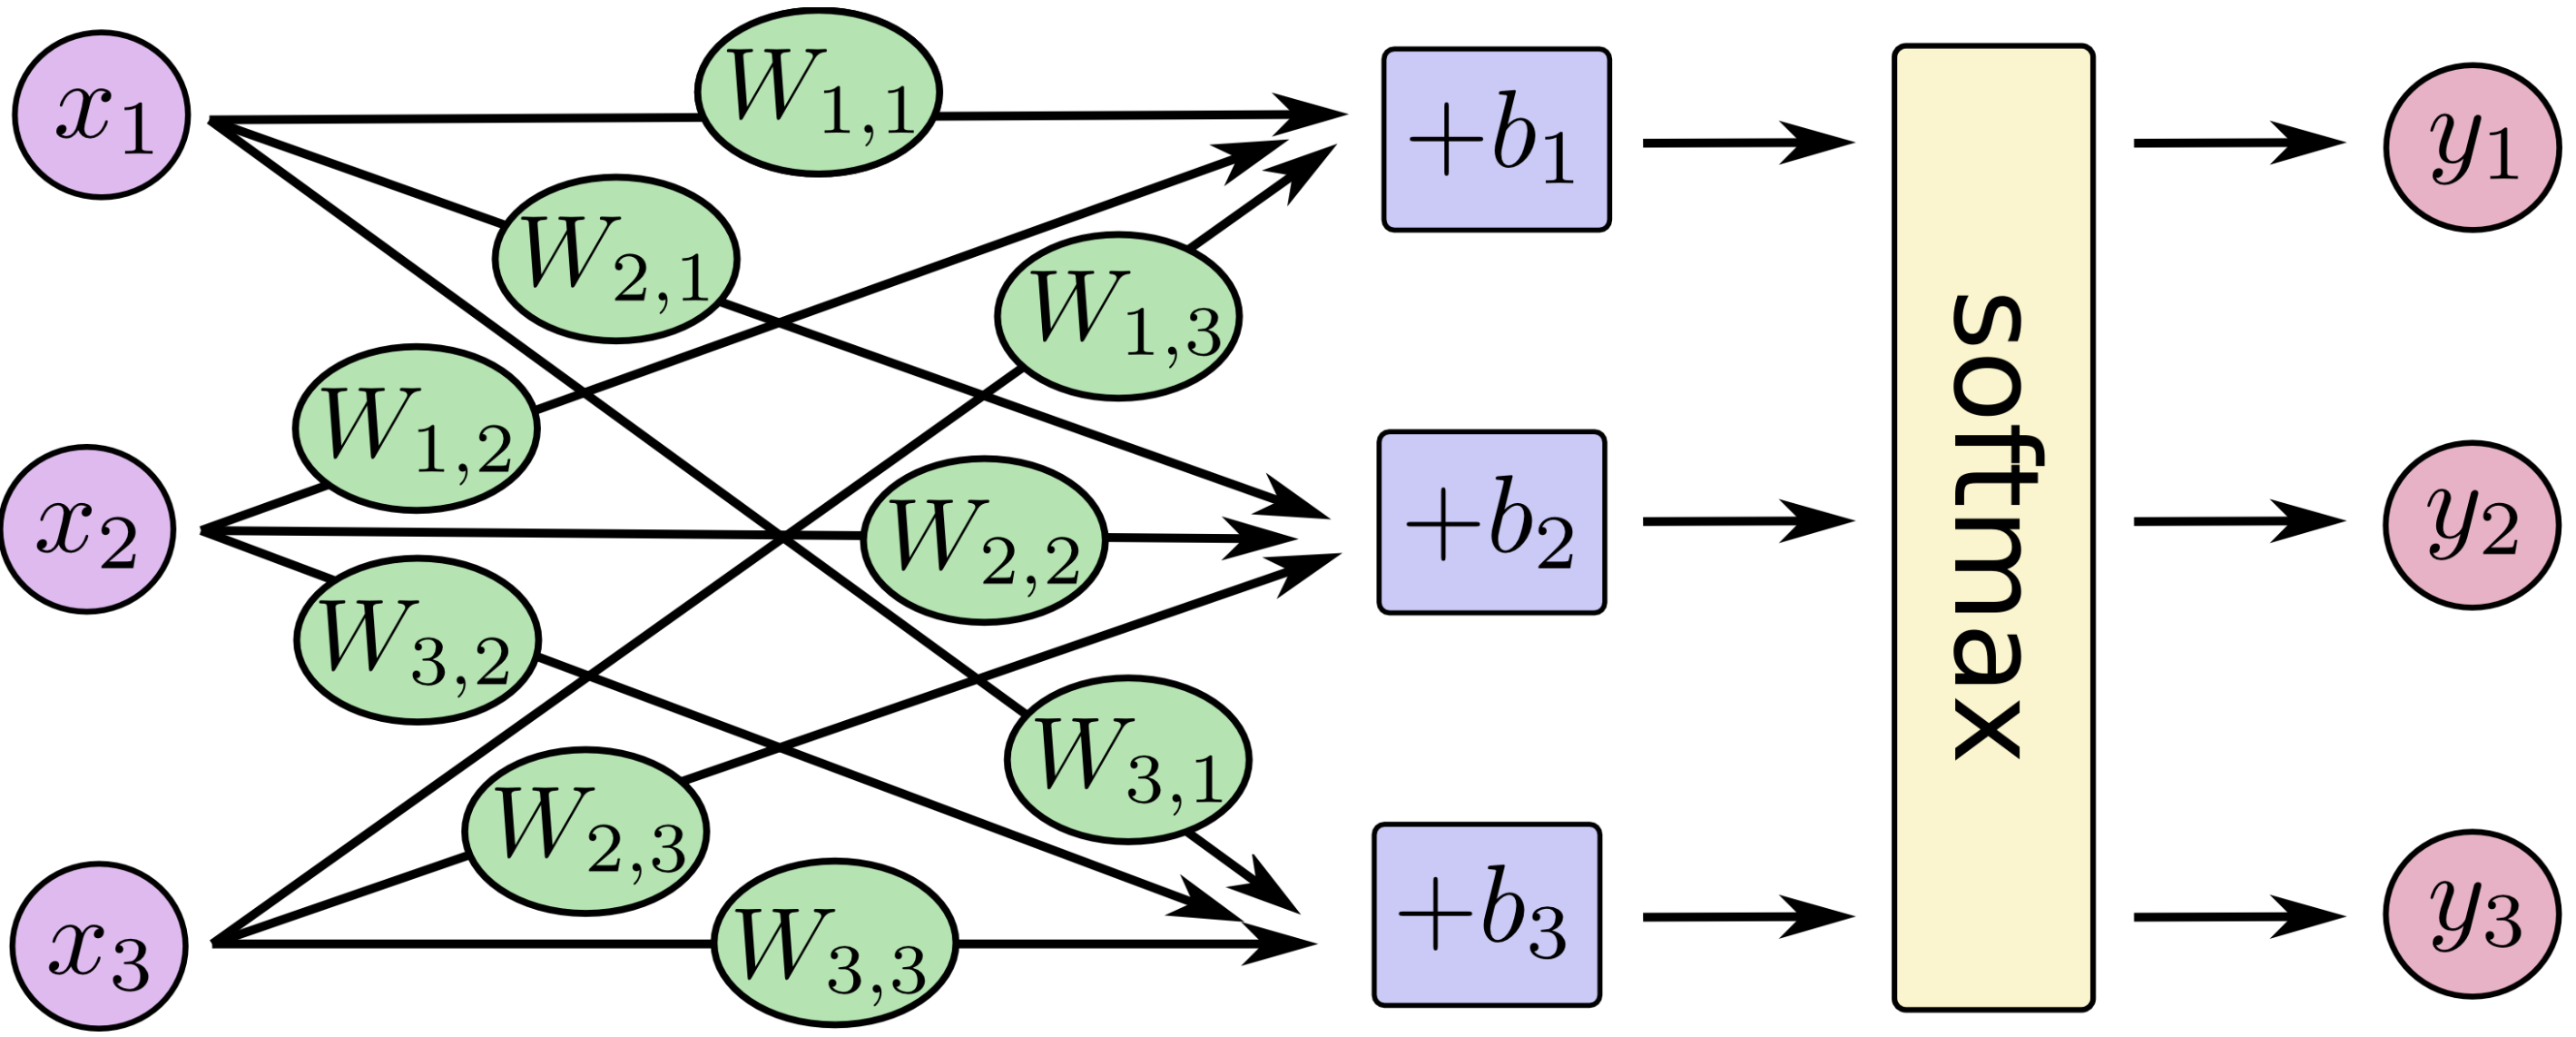
\includegraphics[width=0.4\textwidth]{figures/linear01}

\begin{align}
	\textbf{y}= \textbf{W x} + \textbf{b}
\end{align}	


	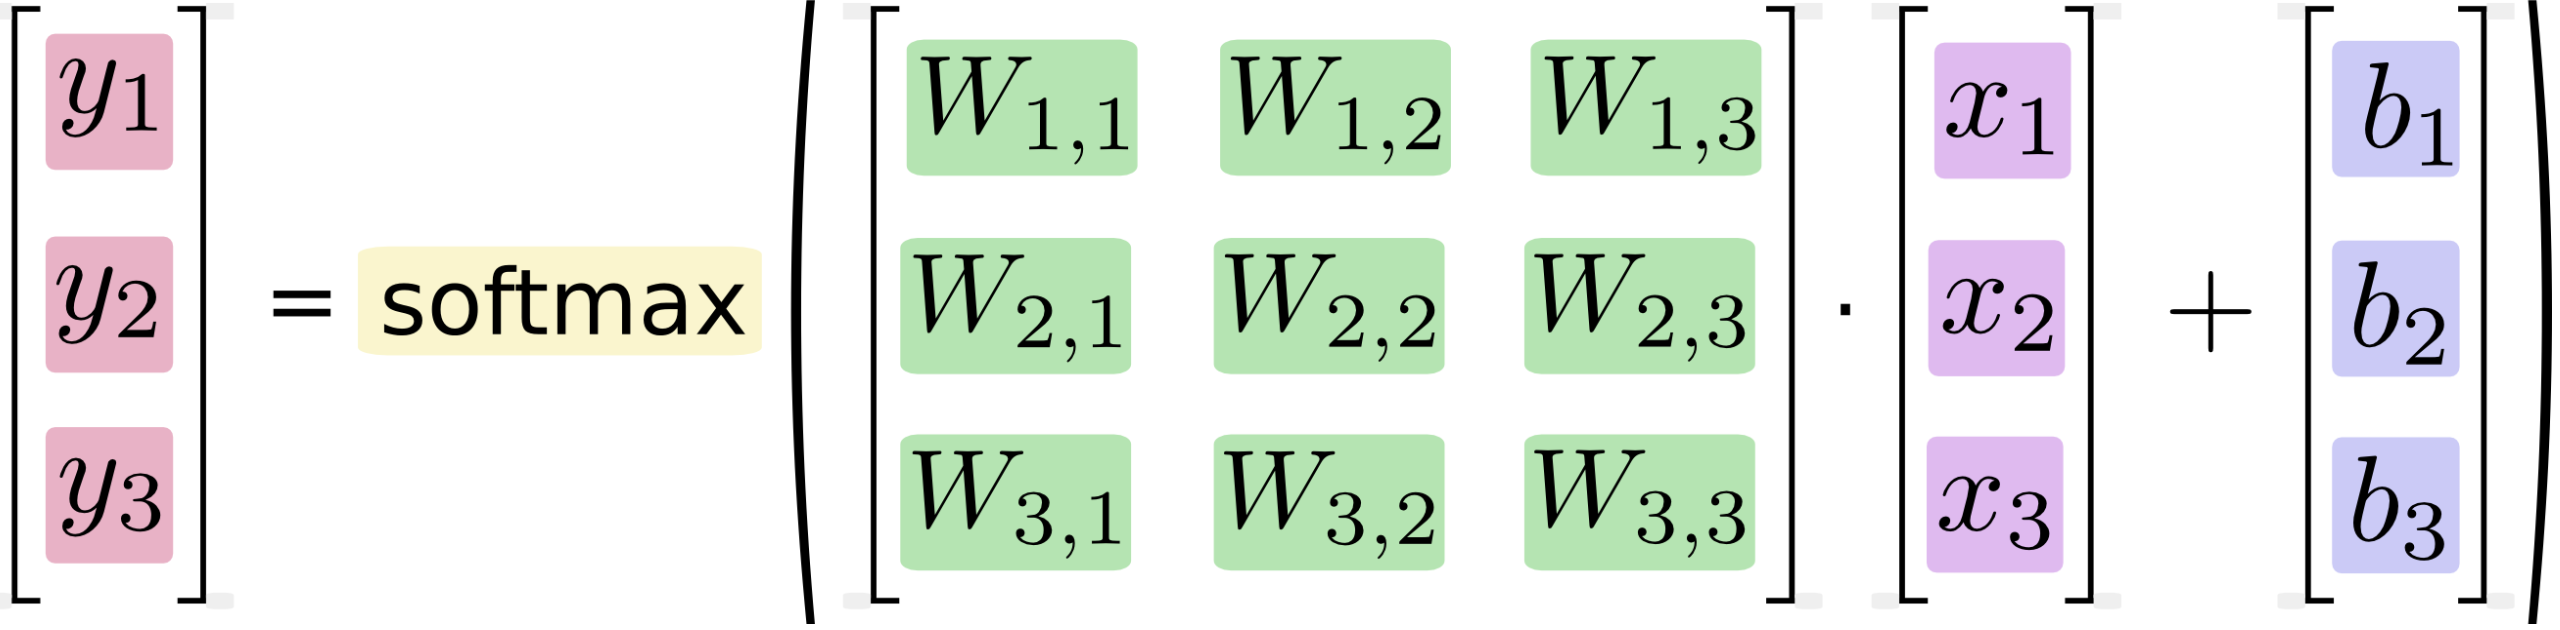
\includegraphics[width=0.4\textwidth]{figures/linear02}

\subsection{Sigmoid Layer}
Sigmoid layer can be used as binary-class classifier with 2-way gating.\\
\textbf{Activation function:} \footnote{For more activation functions see:\\ {\small\url{https://en.wikipedia.org/wiki/Activation_function}}}

\begin{align}
	\sigma(x)=\frac{1}{1+ e^{-x}} = \frac{e^x}{1+e^{x}}
\end{align}

\vspace{-10pt}
\begin{center}
	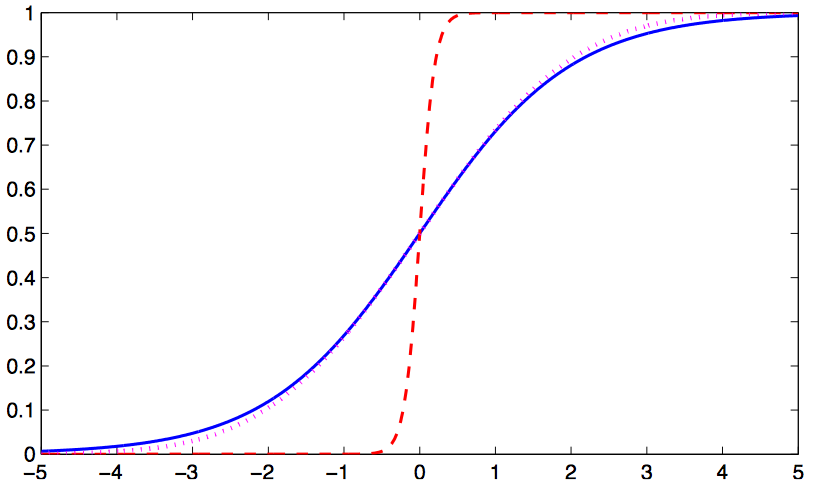
\includegraphics[width=0.4\textwidth]{figures/Sigmoid}
\end{center}


The logistic sigmoid function $\sigma_\beta=1/1+e^{-\beta x} $. The parameter $ \beta $ determines the steepness of the sigmoid. The full (blue) line is for $ \beta=1 $ and the dashed (red) for $ \beta=10 $. As $ \beta \rightarrow \infty $, the logistic sigmoid tends to a Heaviside step function. \\


\textbf{Linear Layer + Sigmoid Layer as a \underline{binary classifier}\\ (Logistirc Regression):}

\begin{align}
	y = f(x) = \sigma(y(x)) = \frac{1}{1+e^{-y}}= \frac{1}{1+e^{-(Wx+b)}}
\end{align}

\begin{center}
	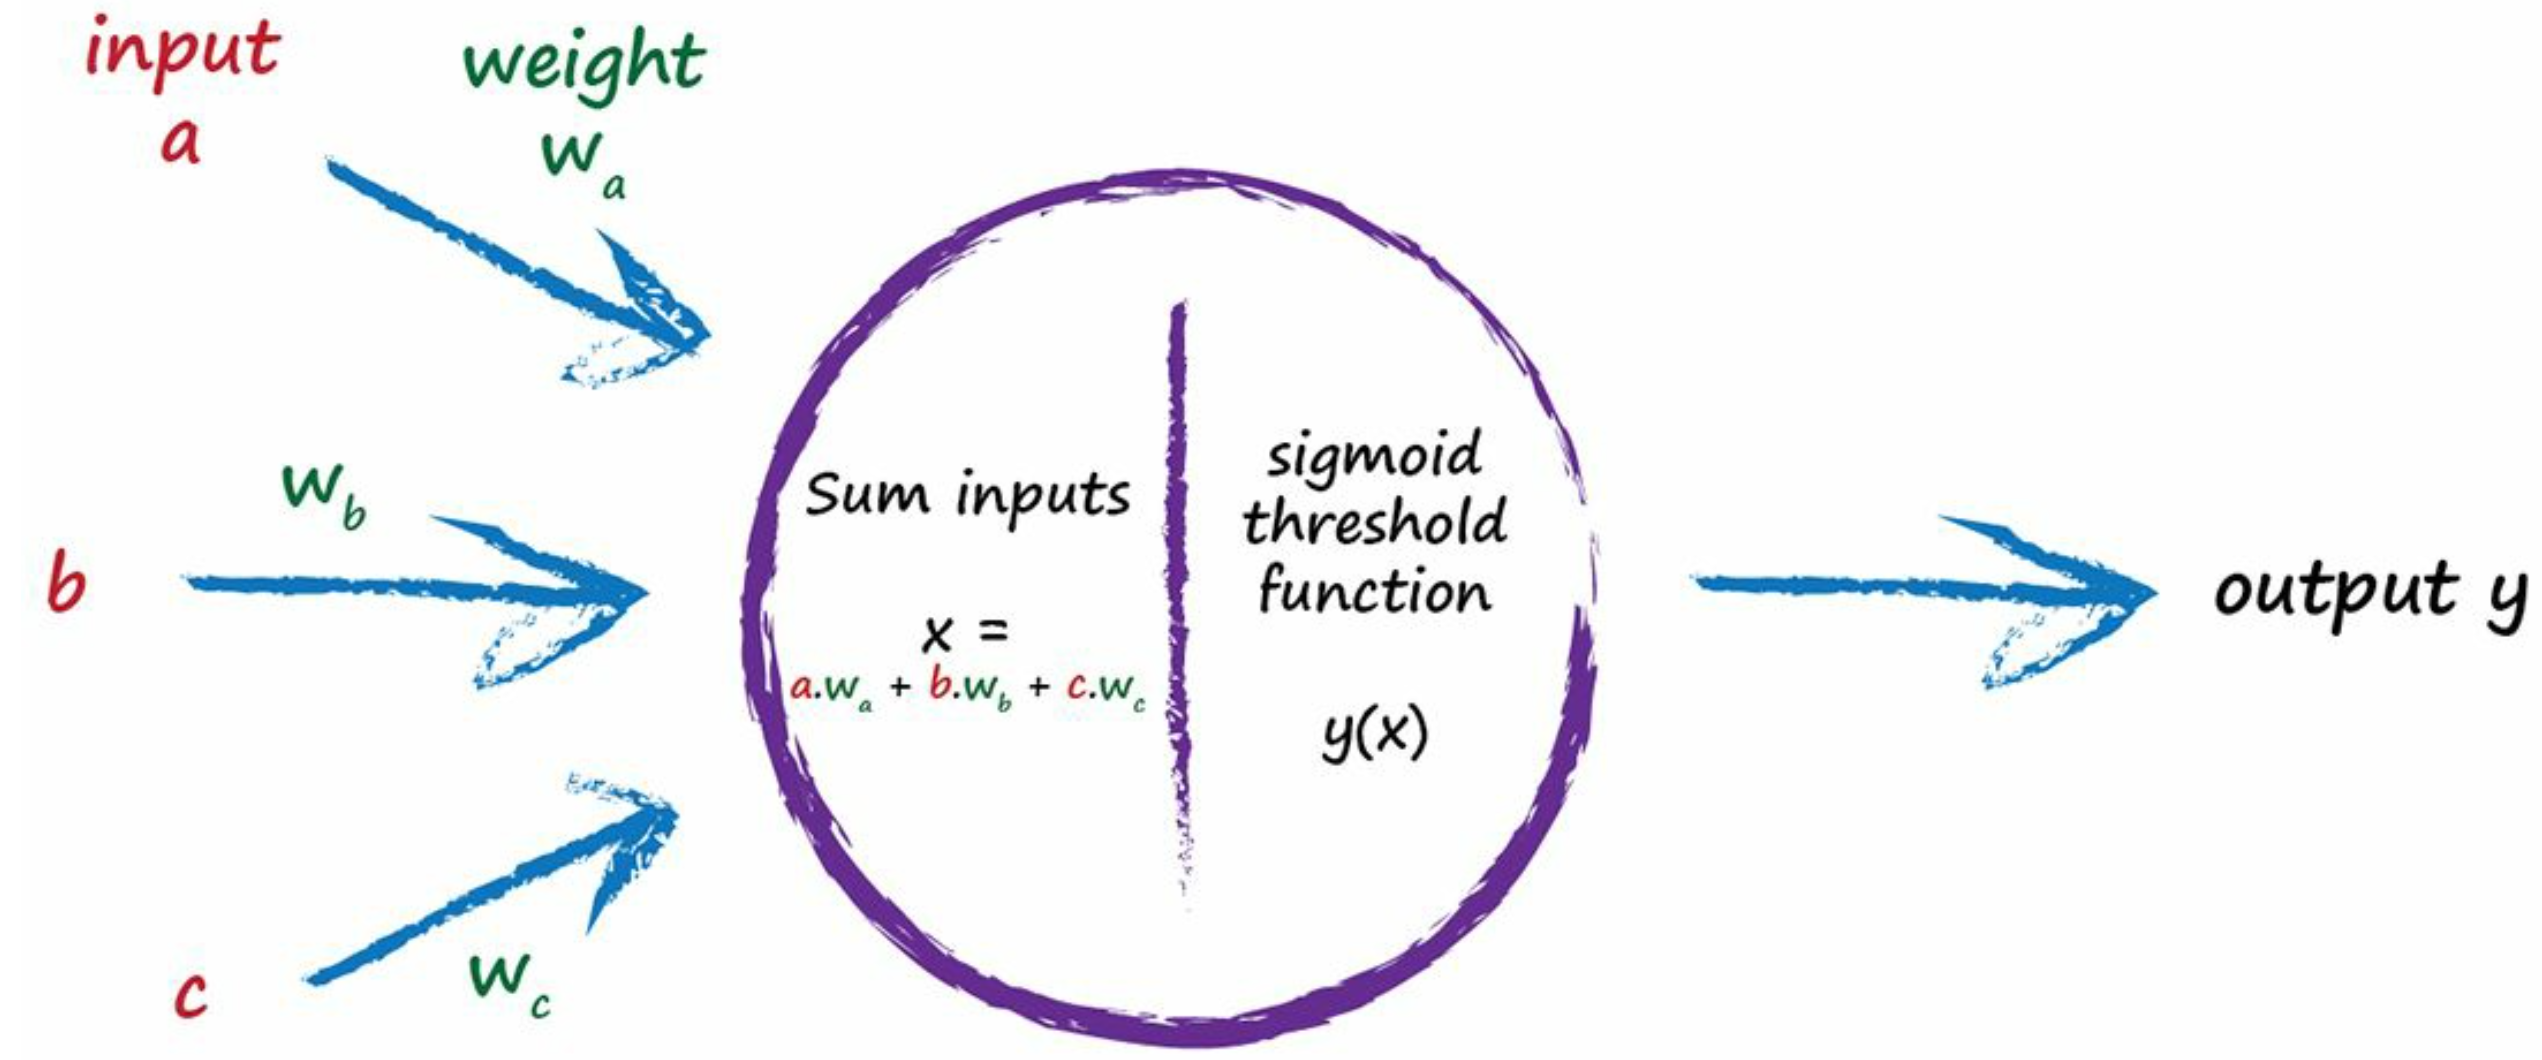
\includegraphics[width=0.55\textwidth]{figures/sigmoid02}
\end{center} 

\textbf{*An alternative activation function is $ \textbf{tanh(x)} $ function:}\\
\vspace{5 pt}
Where $ tanh(x=)f(z) $ here:
\begin{align}
tanh(x)=\frac{e^x-e^{-x}}{e^x+e^{-x}}
\end{align}
\vspace{10pt}
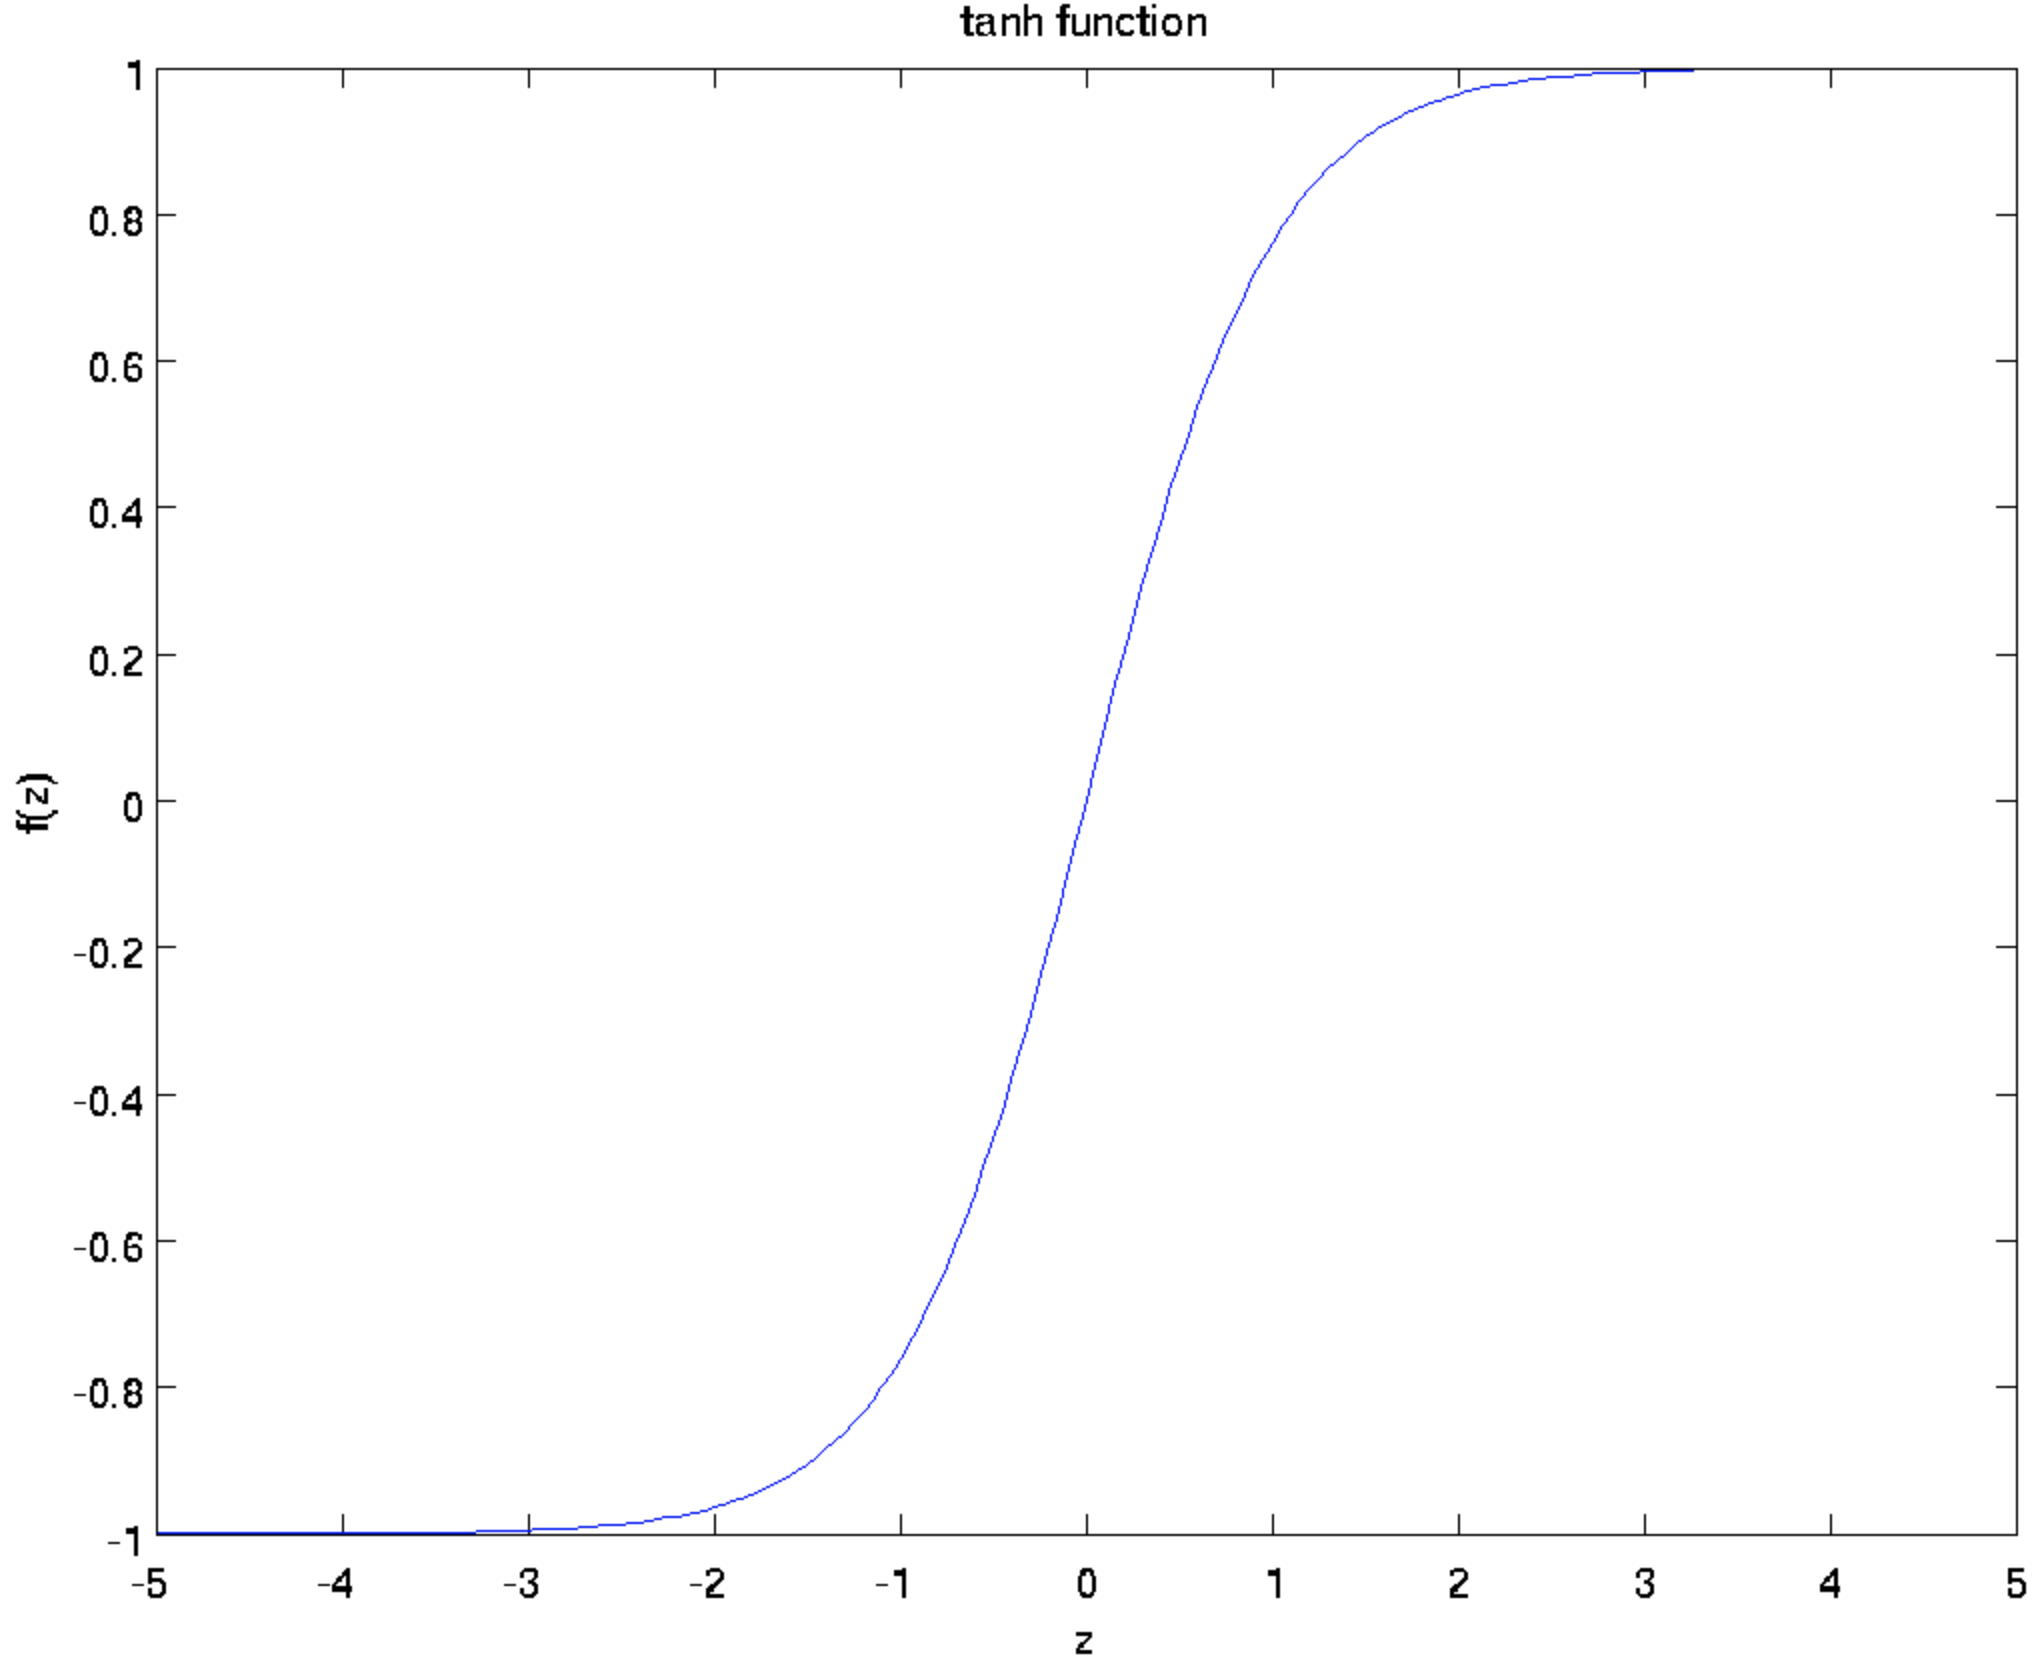
\includegraphics[width=0.55\textwidth]{figures/tanh}

\subsection{Softmax Layer}
Softmax layer can be used as multi-class classification and also in soft/differentiably multi-way gating/routing.

\begin{flalign}
	&&y &= softmax(x)&\\
	&\text{with, }&y_i &=\dfrac{e^{x_i}}{\sum_{j=1}^{K}e^{x_j}}&
\end{flalign}


\textbf{LinearLayer + SoftmaxLayer as a \underline{multi-class classifier}:}\\

\vspace{-10pt}

\begin{align}
	 y_i=\dfrac{e^{\sum_{j}w_{ij}x_i+b_i}}{\sum_{k}e^{\sum_{j}w_{kj}x_j+b_k}} 
\end{align}


\subsection{Rectified-linear Layer (ReLU)}
ReLU is simpler/ cheaper than sigmoid, and it is prevalent in modern neural nets.
\begin{flalign}
	&&y&=ReLU(x) &\\ 
	&\text{with, }&y_i &=max(0, x_i)&
\end{flalign}
%\vspace{-10pt}
\begin{center}
		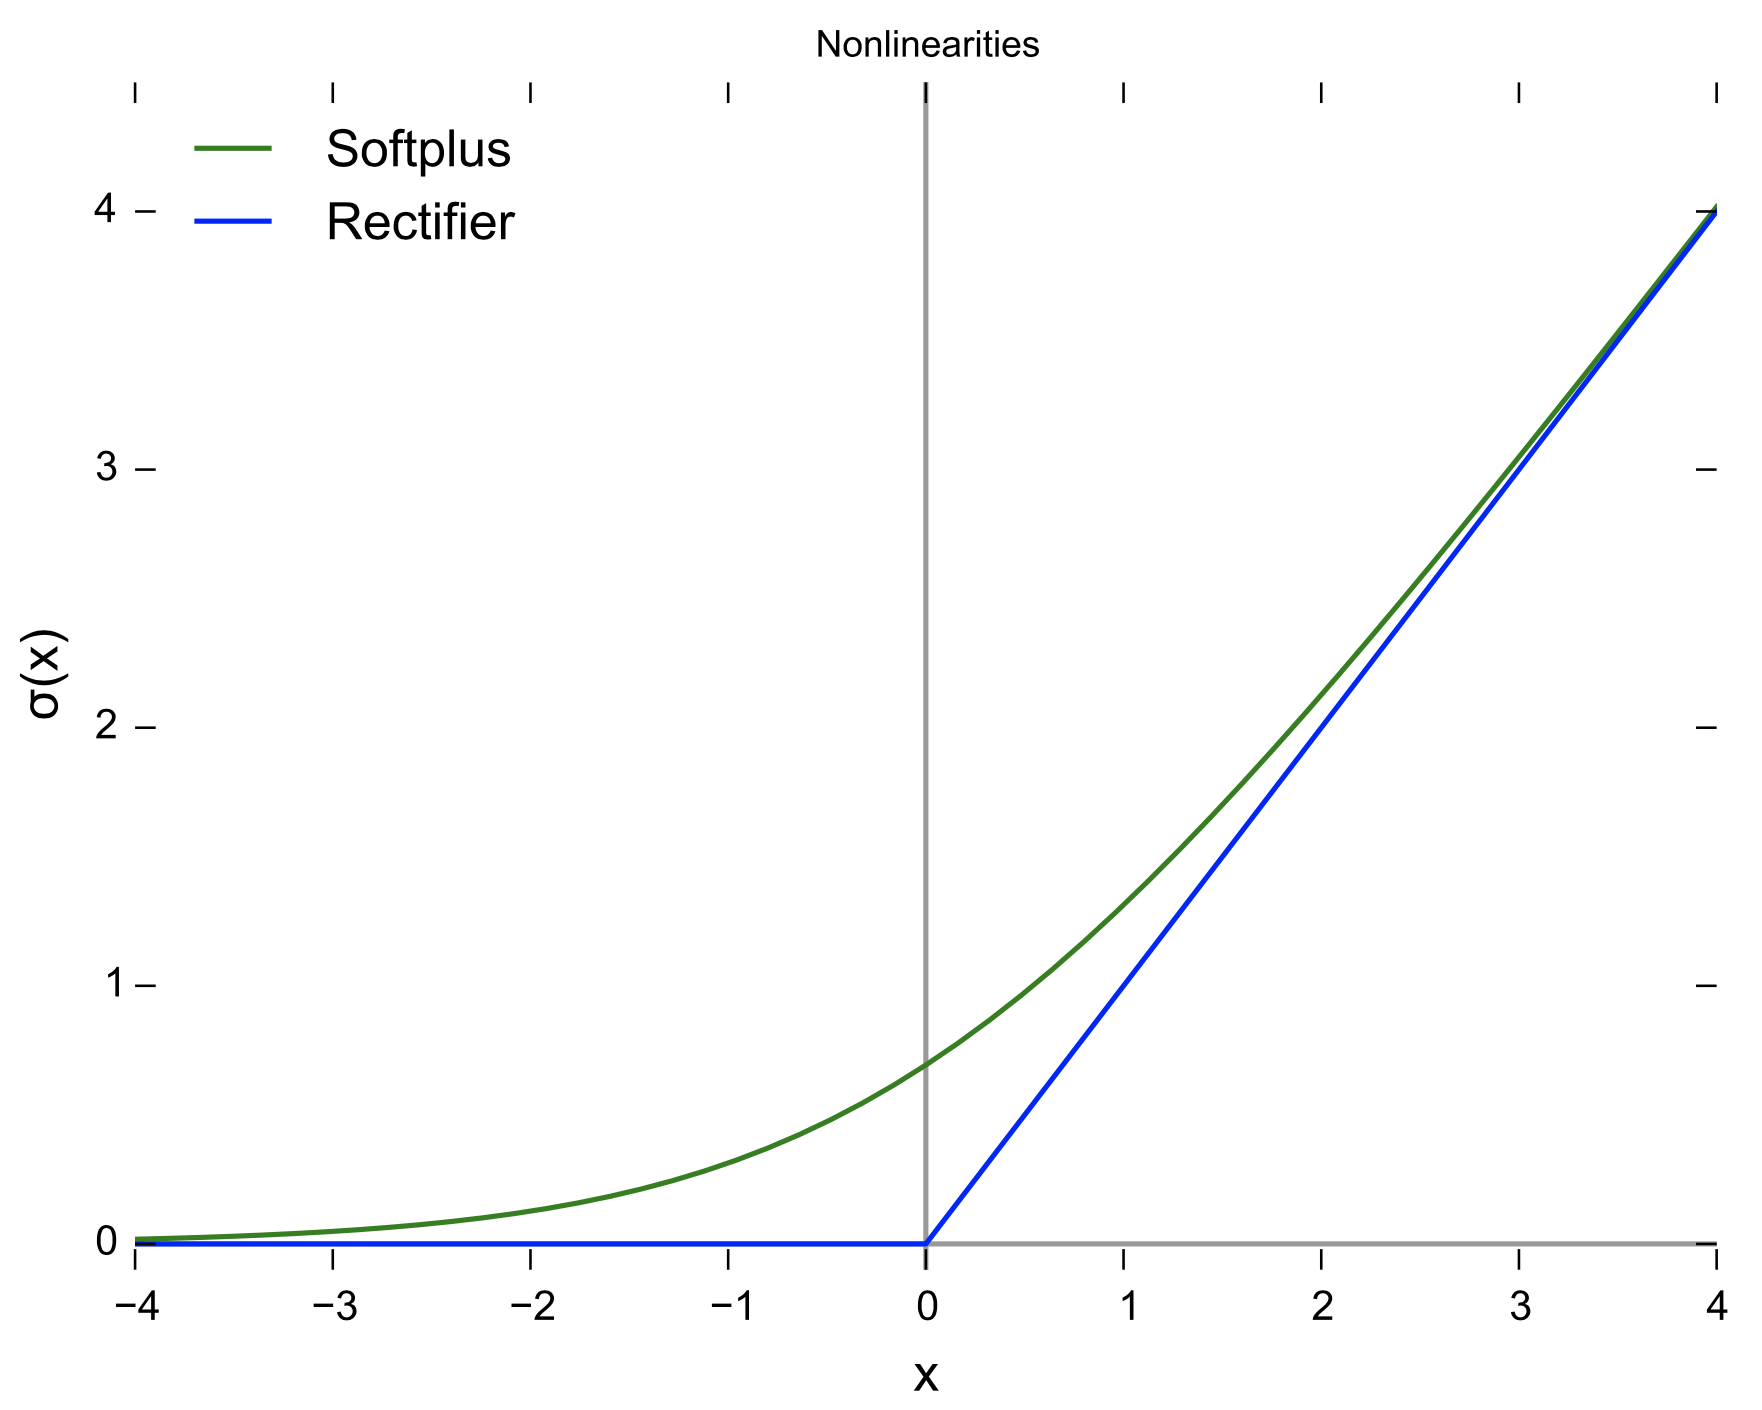
\includegraphics[width=0.35\textwidth]{figures/ReLU}
\end{center}

\subsection{Cross entropy}
Cross-entropy is the 



	\include{chapterOptimization}
	%
	
	\part{Reinforcement  Learning}
	
	\backmatter%%%%%%%%%%%%%%%%%%%%%%%%%%%%%%%%%%%%%%%%%%%%%%%%%%%%%%%
	\appendix
	\include{glossary}
	\printindex
	
	%%%%%%%%%%%%%%%%%%%%%%%%%%%%%%%%%%%%%%%%%%%%%%%%%%%%%%%%%%%%%%%%%%%%%%
	
\end{document}

